%=======================================================================
%  CSE 4112: Machine Learning Laboratory  --  DATASET REPORT
%  Khulna University of Engineering & Technology (KUET)
%
%  Structure follows CSE_4112_Dataset_Report_Template.docx exactly:
%  Page 1 synopsis -> Format block -> Sections 1-17 -> Appendices A, B, C
%
%  Compile with pdfLaTeX (default on Overleaf). No shell-escape needed.
%  For Bangla script in the body, compile with XeLaTeX and uncomment the
%  polyglossia block marked [BANGLA] below.
%=======================================================================
\documentclass[11pt,a4paper]{article}

%---------------------------------------------------------------- fonts
\usepackage[T1]{fontenc}
\usepackage[utf8]{inputenc}
\usepackage{mathptmx}                 % Times New Roman body (11 pt)
\usepackage[scaled=0.92]{helvet}      % Arial-like headings/figures
\usepackage{courier}

%------------------------------------------------------------ page setup
\usepackage[a4paper,margin=20mm,headheight=14pt]{geometry}
\usepackage{setspace}
\setstretch{1.15}                     % 1.15 line spacing
\setlength{\parskip}{6pt plus 1pt}    % 6 pt after body paragraphs
\setlength{\parindent}{0pt}

%------------------------------------------------------------- packages
\usepackage{etoolbox}
\usepackage{graphicx}
\usepackage{booktabs}
\usepackage{array}
\usepackage{longtable}
\usepackage{tabularx}
\usepackage{multirow}
\usepackage{enumitem}
\usepackage{caption}
\usepackage{xcolor}
\usepackage{amssymb}
\usepackage{fancyhdr}
\usepackage{titlesec}
\usepackage[hidelinks,breaklinks]{hyperref}
\usepackage{url}
% Allow the repository URL to wrap inside narrow table columns.
\def\UrlBreaks{\do\/\do\-\do\.\do\_\do\a\do\b\do\c\do\d\do\e\do\f%
  \do\g\do\h\do\i\do\j\do\k\do\l\do\m\do\n\do\o\do\p\do\q%
  \do\r\do\s\do\t\do\u\do\v\do\w\do\x\do\y\do\z}
\Urlmuskip=0mu plus 1mu


%------------------------------------------------ [BANGLA] XeLaTeX only
% \usepackage{polyglossia}
% \setdefaultlanguage{english}
% \setotherlanguage{bengali}
% \newfontfamily\bengalifont[Script=Bengali]{Noto Sans Bengali}
% Usage:  \textbengali{...}
%-----------------------------------------------------------------------

%------------------------------------------- long paths in narrow columns
% \texttt{} file paths cannot hyphenate, which overfills narrow table cells.
% hyphenat's htt option lets monospace text break; emergencystretch gives TeX
% slack before it gives up on a line.
\usepackage[htt]{hyphenat}

%--------------------------------------------------- TikZ flow diagrams (page 1)
\usepackage{tikz}
\usetikzlibrary{arrows.meta,positioning,calc,fit,backgrounds}
\definecolor{cAsk}{HTML}{E7EAF0}\definecolor{cAskB}{HTML}{6B7483}
\definecolor{cSig}{HTML}{DCE8F6}\definecolor{cSigB}{HTML}{3E6FA8}
\definecolor{cDat}{HTML}{DDEEE1}\definecolor{cDatB}{HTML}{3C7D52}
\definecolor{cMod}{HTML}{FBE6D4}\definecolor{cModB}{HTML}{B5701F}
\definecolor{cOut}{HTML}{EAE1F2}\definecolor{cOutB}{HTML}{6E4B9E}
\tikzset{
  fbox/.style={draw, line width=0.6pt, rounded corners=2.5pt, align=flush center,
               inner sep=3pt, font=\sffamily\scriptsize, text width=#1},
  farr/.style={-{Stealth[length=2.2mm,width=1.9mm]}, line width=0.8pt, draw=black!50},
  fnum/.style={circle, draw=black!45, fill=white, line width=0.4pt, inner sep=0pt,
               minimum size=3.4mm, font=\sffamily\bfseries\tiny},
  band/.style={rounded corners=3pt, draw=black!18, line width=0.5pt, fill=black!3},
  bandlbl/.style={font=\sffamily\bfseries\tiny, text=black!55},
}
\newcommand{\fhd}[1]{\textbf{#1}\\[1.5pt]}

\setlength{\emergencystretch}{3em}

%----------------------------------------------------- heading styles
\titleformat{\section}{\sffamily\bfseries\large}{\thesection.}{0.6em}{}
\titleformat{\subsection}{\sffamily\bfseries\normalsize}{\thesubsection}{0.6em}{}
\titlespacing*{\section}{0pt}{12pt}{6pt}
\titlespacing*{\subsection}{0pt}{10pt}{4pt}
\renewcommand{\thesection}{\arabic{section}}

% captions: Arial, self-explanatory, single-spaced
\captionsetup{font={sf,small,singlespacing},labelfont=bf,skip=4pt}

%-------------------------------------------------------- table helpers
\renewcommand{\arraystretch}{1.25}
\newcolumntype{L}[1]{>{\raggedright\arraybackslash}p{#1}}
\newcolumntype{Y}{>{\raggedright\arraybackslash}X}
\newcommand{\thd}[1]{\textbf{\sffamily\small #1}}          % table header
\newcommand{\ph}[1]{\textcolor{gray}{[#1]}}                % placeholder
\newcommand{\yn}{$\square$~Yes~/~$\square$~No}             % checklist cell
\newcommand{\arr}{\;$\rightarrow$\;}

% single-spacing inside tables
\AtBeginEnvironment{tabular}{\setstretch{1.0}\small}
\AtBeginEnvironment{tabularx}{\setstretch{1.0}\small}
\AtBeginEnvironment{longtable}{\setstretch{1.0}\small}

%--------------------------------------------------------------- header
\pagestyle{fancy}
\fancyhf{}
\fancyhead[L]{\sffamily\footnotesize CSE 4112: Machine Learning Laboratory}
\fancyhead[R]{\sffamily\footnotesize Dataset Report}
\fancyfoot[C]{\sffamily\footnotesize\thepage}
\renewcommand{\headrulewidth}{0.4pt}

%=======================================================================
\begin{document}

%=======================================================================
%  PAGE 1 -- VISUAL SYNOPSIS  (keep to exactly one page)
%=======================================================================
\thispagestyle{empty}
\begin{center}
  % 
\includegraphics[width=22mm]{figures/kuet_logo.png}\\[4pt]
  {\sffamily\large\bfseries Khulna University of Engineering \& Technology}\\[2pt]
  {\sffamily Department of Computer Science and Engineering}\\[2pt]
  {\sffamily CSE 4112: Machine Learning Laboratory}\\[10pt]
  {\sffamily\LARGE\bfseries DATASET REPORT}\\[8pt]
  {\large\bfseries A Speaker-Attributed Sentiment Dataset for\\
   Bangla Financial Television Talk Shows}\\[10pt]
\end{center}

\begin{center}
\begin{tabularx}{\textwidth}{|L{2.2cm}|Y|L{2.6cm}|Y|}
\hline
\thd{Group No.}  & \textbf{1}
& \thd{Dataset Version} & v1.0 (15 September 2026) \\ \hline
\thd{Students}   & \small Nafiz Ahmed (2107001) \textbullet{} Tawhidul Hasan (2107004) \textbullet{} Sarwad Hasan Siddiqui (2107006) \textbullet{} Saif Ahmed Shejan (2107009) \textbullet{} Maruf Shafiq (2107010) \textbullet{} Dewan Salman Rahman Zisan (2107015)
& \thd{Repository}      & {\scriptsize\url{https://github.com/mayer-doa-coder/bangla-financial-talkshow-sentiment}} \\ \hline
\end{tabularx}
\end{center}

\vspace{4pt}
{\sffamily\bfseries What the dataset makes possible}
\vspace{1pt}

\begin{center}
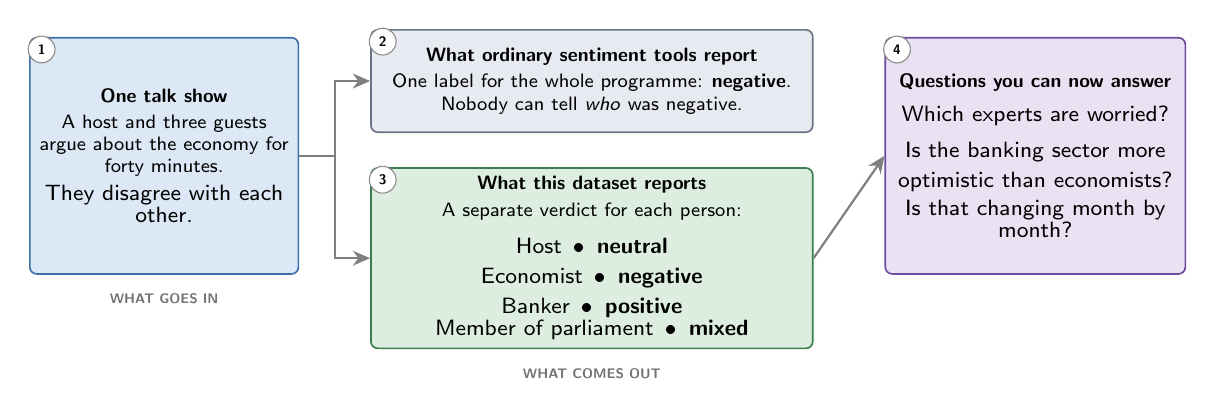
\begin{tikzpicture}[node distance=0mm]
% ---------------------------------------------------------------- input
\node[fbox=32mm, fill=cSig, draw=cSigB, minimum height=30mm] (g1)
  {\fhd{One talk show}
   A host and three guests argue about the economy for forty minutes.
   \\[2pt]
   {\footnotesize They disagree with each other.}};

% ------------------------------------------------- the usual answer (top)
\node[fbox=54mm, fill=cAsk, draw=cAskB, minimum height=13mm,
      right=9mm of g1, yshift=9.5mm] (g2)
  {\fhd{What ordinary sentiment tools report}
   One label for the whole programme: \textbf{negative}.
   Nobody can tell \emph{who} was negative.};

% ------------------------------------------------ what this dataset adds
\node[fbox=54mm, fill=cDat, draw=cDatB, minimum height=22mm,
      right=9mm of g1, yshift=-13mm] (g3)
  {\fhd{What this dataset reports}
   A separate verdict for each person:
   \\[2.5pt]
   {\footnotesize\setstretch{1.15}
   Host \,\textbullet\, \textbf{neutral} \\
   Economist \,\textbullet\, \textbf{negative} \\
   Banker \,\textbullet\, \textbf{positive} \\
   Member of parliament \,\textbullet\, \textbf{mixed}}};

% ---------------------------------------------------------------- output
\node[fbox=36mm, fill=cOut, draw=cOutB, minimum height=30mm,
      right=9mm of g3.east, anchor=west, yshift=13mm] (g4)
  {\fhd{Questions you can now answer}
   {\footnotesize\setstretch{1.15}
   Which experts are worried? \\[2pt]
   Is the banking sector more
   optimistic than economists? \\[2pt]
   Is that changing month by month?}};

\draw[farr] (g1.east) -- ++(4.5mm,0) |- (g2.west);
\draw[farr] (g1.east) -- ++(4.5mm,0) |- (g3.west);
\draw[farr] (g3.east) -- (g4.west);

\foreach \n/\k in {g1/1, g2/2, g3/3, g4/4}
  \node[fnum] at ($(\n.north west)+(1.6mm,-1.6mm)$) {\k};
\node[bandlbl, below=1.2mm of g1] {WHAT GOES IN};
\node[bandlbl, below=1.2mm of g3] {WHAT COMES OUT};
\end{tikzpicture}
\end{center}

{\sffamily\small\setstretch{1.0}\textbf{Figure 1.} The idea in one picture. Existing Bangla
sentiment resources label a document or a sentence, so a programme in which four people disagree
collapses into a single score. This dataset keeps the speakers apart and gives each one a verdict
for the episode, which is what makes it possible to ask who holds which position rather than only
how the programme sounded overall.\par}

\vspace{10pt}
{\sffamily\bfseries The dataset at a glance}
\vspace{3pt}

\begin{center}
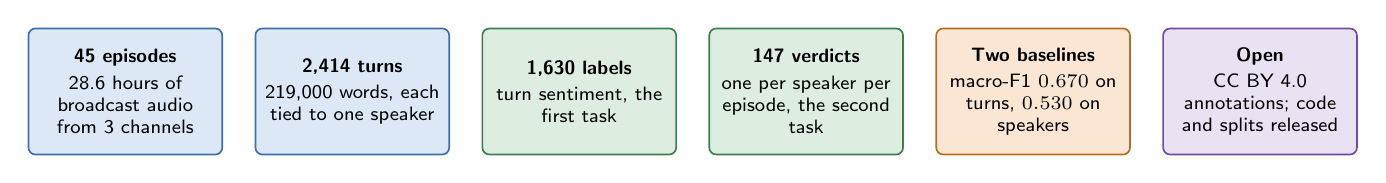
\begin{tikzpicture}[node distance=0mm]
\def\gw{22.5mm}
\node[fbox=\gw, fill=cSig, draw=cSigB, minimum height=16mm] (n1)
  {\fhd{45 episodes} 28.6 hours of broadcast audio from 3 channels};
\node[fbox=\gw, fill=cSig, draw=cSigB, minimum height=16mm, right=4mm of n1] (n2)
  {\fhd{2{,}414 turns} 219{,}000 words, each tied to one speaker};
\node[fbox=\gw, fill=cDat, draw=cDatB, minimum height=16mm, right=4mm of n2] (n3)
  {\fhd{1{,}630 labels} turn sentiment, the first task};
\node[fbox=\gw, fill=cDat, draw=cDatB, minimum height=16mm, right=4mm of n3] (n4)
  {\fhd{147 verdicts} one per speaker per episode, the second task};
\node[fbox=\gw, fill=cMod, draw=cModB, minimum height=16mm, right=4mm of n4] (n5)
  {\fhd{Two baselines} macro-F1 $0.670$ on turns, $0.530$ on speakers};
\node[fbox=\gw, fill=cOut, draw=cOutB, minimum height=16mm, right=4mm of n5] (n6)
  {\fhd{Open} CC BY 4.0 annotations; code and splits released};
\end{tikzpicture}
\end{center}

{\sffamily\small\setstretch{1.0}Every label in this release was written by a language model
following a rubric the team wrote, and then checked for internal consistency; no human annotator
re-labelled individual turns. Scores therefore measure agreement with that judge rather than with
human ground truth, and the report says so wherever a number appears.\par}



\clearpage

%=======================================================================
\section*{\sffamily REPORT PREPARATION AND SUBMISSION FORMAT}
%=======================================================================

This is a course-specific dataset report template. It combines the reporting logic of
\emph{Data in Brief} with common data-descriptor elements used by \emph{Scientific Data} and
\emph{MDPI Data}, and adds an ML-readiness/baseline section for CSE 4112.

\begin{tabularx}{\textwidth}{|L{3.4cm}|Y|}
\hline
\thd{Paper \& margins}      & A4 (210 $\times$ 297 mm); approximately 20 mm margins. \\ \hline
\thd{Font}                  & Times New Roman, 11 pt body; Arial for headings/figures. Keep formatting consistent. \\ \hline
\thd{Spacing}               & 1.15 line spacing; 6 pt after body paragraphs. Single spacing is acceptable in tables/captions. \\ \hline
\thd{Recommended length}    & About 8--12 pages after Page 1, excluding appendices. Quality and completeness are more important than page count. \\ \hline
\thd{Figures \& tables}     & Number consecutively; cite every figure/table in the text; captions must be self-explanatory. \\ \hline
\thd{References}            & Numbered citation style in square brackets. Prefer dataset papers, data-collection sources, instruments/software, and relevant ML references. \\ \hline
\thd{Submission files}      & One report (DOCX/PDF as instructed), dataset/repository link, README, data dictionary, and code/notebook link where applicable. \\ \hline
\end{tabularx}

%=======================================================================
\section{Dataset Article Information}
%=======================================================================

\begin{tabularx}{\textwidth}{|L{4.2cm}|Y|}
\hline
\thd{Dataset/report title}  & A Speaker-Attributed Sentiment Dataset for Bangla Financial Television Talk Shows \\ \hline
\thd{Group and students}    & Group 1; six students: Nafiz Ahmed (2107001), Tawhidul Hasan (2107004), Sarwad Hasan Siddiqui (2107006), Saif Ahmed Shejan (2107009), Maruf Shafiq (2107010), Dewan Salman Rahman Zisan (2107015) \\ \hline
\thd{Affiliation}           & Department of CSE, KUET, Khulna-9203, Bangladesh \\ \hline
\thd{Corresponding student} & Tawhidul Hasan (2107004), hasan2107004@stud.kuet.ac.bd \\ \hline
\thd{Keywords}              & Bangla NLP; speaker-level sentiment; financial talk shows; speaker diarization; automatic speech recognition; LLM-as-judge; BanglaBERT; low-resource corpus \\ \hline
\thd{Dataset version}       & v1.0; released 15 September 2026 \\ \hline
\thd{Repository / persistent ID} & Git repository: {\scriptsize\url{https://github.com/mayer-doa-coder/bangla-financial-talkshow-sentiment}}. Access is currently restricted to the course instructor and the authors; no DOI is minted yet. Source broadcast audio and the fine-tuned checkpoint are excluded; see Section 13 and the repository \texttt{.gitignore}. \\ \hline
\thd{License}               & CC BY 4.0 for the derived annotations, transcripts and timings \emph{only}. Source broadcast audio is third-party copyrighted and is not covered by this licence and not redistributed (Section 13). \\ \hline
\thd{Related article / source} & None \\ \hline
\end{tabularx}

%=======================================================================
\section{Abstract}
%=======================================================================

\emph{\small Write 150--300 words. Describe why the dataset was created, how data were
collected/compiled, what the dataset contains, its scale/formats, quality-control approach, and
how it may be reused. Do not turn the abstract into a results or conclusion section.}

Bangla financial television talk shows carry the evaluative positions of economists, bankers,
industrialists and regulators, but existing Bangla sentiment resources are built from
social-media text and score whole documents rather than individual speakers. This dataset was
created to make \emph{who holds which position} machine-readable. Forty-five unique episodes
(approximately 28.6 hours) from Bangladeshi business talk shows were processed through a
reproducible pipeline: audio hygiene and voice-activity detection, \texttt{pyannote} speaker
diarization, Whisper-medium Bangla ASR, and word-level fusion of the two streams. Fusion output
was merged from fixed ASR decode windows back into 2{,}414 coherent speaker turns across 212
speaker--episode units. Because no human sentiment labels existed for this genre, labels were
produced by a large-language-model judge operating under a published rubric that separates
evaluative stance from emotion, treats a host's pointed question as elicitation rather than
assertion, and allows an explicit \texttt{illegible} class for turns the ASR destroyed. The
release contains 2{,}414 turns, 150 judged speaker units, 1{,}811 turn labels and 1{,}630
supervised turns partitioned episode-disjointly into 1{,}009/297/324. A BanglaBERT baseline reaches
a test turn-level macro-F1 of 0.670 ($\kappa=0.496$) against a majority-class floor of 0.236 and a
TF--IDF reference of 0.529, and a hierarchical speaker model scores 0.530 macro-F1 in grouped
cross-validation over all 147 speaker units, demonstrating that the corpus supports a valid
supervised workflow at both levels. \textbf{All reported scores measure
agreement with the judge, not with human ground truth}; word error rate, diarization error rate
and annotator agreement remain unmeasured and are documented as such.

%=======================================================================
\section{Dataset Specifications Table}
%=======================================================================

\begin{longtable}{|L{4.0cm}|L{11.4cm}|}
\hline
\thd{Item} & \thd{Required information} \\ \hline
\endfirsthead
\hline \thd{Item} & \thd{Required information} \\ \hline \endhead
\thd{Subject / domain}          & Computer science and natural language processing; applied economics / financial media analysis \\ \hline
\thd{Specific subject area}     & Speaker-attributed sentiment and stance analysis of Bangla-language broadcast financial discourse \\ \hline
\thd{Type of data}              & Multimodal: raw broadcast audio (not redistributed), processed WAV, ASR transcripts, diarization segments, fused word--speaker alignments, speaker turns, and sentiment labels. Both raw and processed components are released. \\ \hline
\thd{File formats}              & MP3/MPEG (source), WAV 16 kHz mono (processed), JSON (ASR, diarization, fusion), RTTM (diarization, standard), JSONL (turns, speakers, labels, splits), CSV (registry, lexicons), Jupyter \texttt{.ipynb} \\ \hline
\thd{Unit of observation}       & One \textbf{speaker turn}: a maximal run of consecutive ASR decode windows attributed to the same speaker within one episode. A secondary unit is the \textbf{speaker--episode unit} (all turns by one speaker in one episode). \\ \hline
\thd{Data collection / source}  & Secondary compilation: publicly broadcast television talk-show recordings collected by six students, then processed by an automatic pipeline. Sentiment labels are primary annotations generated by an LLM judge. \\ \hline
\thd{Instrument / software}     & \texttt{pyannote/speaker-diarization-community-1} (rev \texttt{3533c8cf}) with \texttt{wespeaker-voxceleb-resnet34-LM} embeddings; \texttt{bengaliAI/tugstugi\_bengaliai-asr\_whisper-medium} (rev \texttt{da605cc1}) via CTranslate2; \texttt{csebuetnlp/banglabert} (rev \texttt{9ce791f3}); Claude Opus 5 judge; PyTorch 2.12, \texttt{transformers}, \texttt{scikit-learn} \\ \hline
\thd{Data source location}      & Bangladesh; Bangla-language national business/economics television programmes (ATN Bangla, RTV Business, Desh TV, GTV, Kaler Kantho, Star News, Dhaka Stream and others) \\ \hline
\thd{Collection period}         & Original broadcast dates are \textbf{not recorded} in the source postings and are therefore not claimed; \texttt{registry.csv} carries channel, title and duration but no air date. Episodes were retrieved from public platform postings and the pipeline runs were executed August--September 2026 (second build). \\ \hline
\thd{Dataset size}              & 45 unique episodes ($\approx$28.6 h audio); 5{,}327 ASR decode windows; \textbf{2{,}414 speaker turns} ($\approx$219{,}000 words); 212 speaker--episode units; 150 judged units; 1{,}811 turn labels; 1{,}630 supervised turns \\ \hline
\thd{Target / labels}           & Turn level: \{\texttt{negative}, \texttt{neutral}, \texttt{positive}\} (plus \texttt{illegible}, excluded from supervision). Speaker level: \{\texttt{negative}, \texttt{mixed}, \texttt{neutral}, \texttt{positive}\} plus a continuous \texttt{stance\_score} $\in[-1,1]$. \\ \hline
\thd{Accessibility}             & Git repository (restricted at submission): {\scriptsize\url{https://github.com/mayer-doa-coder/bangla-financial-talkshow-sentiment}}. It carries the derived annotations, transcripts, timings, diarization output, the build and baseline code and this report; the source broadcast audio is not redistributed. \\ \hline
\thd{License / reuse terms}     & CC BY 4.0 for the derived annotations; source broadcast audio is third-party copyrighted and is \textbf{not} redistributed; see Section 13. \\ \hline
\end{longtable}
% This longtable has no caption, so it must not consume a table number.
\addtocounter{table}{-1}

%=======================================================================
\section{Value of the Data}
%=======================================================================

\emph{\small Provide 3--6 concise bullet points. Explain why the data are useful, who can reuse
them, what research/engineering questions they can support, and what makes the dataset
practically relevant. Avoid unsupported claims of novelty or superiority.}

\begin{itemize}[leftmargin=1.4em,itemsep=2pt,topsep=2pt]
  \item The data attach sentiment to \textbf{individual speakers} rather than to whole episodes.
        In a panel discussion the host, the economist and the industry representative frequently
        disagree; a document-level label averages that disagreement away and discards exactly the
        information a financial sentiment signal needs.
  \item The corpus is a rare Bangla resource in the \textbf{spoken, broadcast, financial} domain.
        Published Bangla sentiment datasets are overwhelmingly written social-media text, so this
        release supports questions about domain shift from written to ASR-transcribed speech.
  \item It supports several ML tasks directly: turn-level sentiment classification, speaker-level
        stance aggregation, role classification (host vs.\ guest), hierarchical document modelling
        over speaker scripts, and robustness studies on noisy ASR output.
  \item Every intermediate artefact is preserved: diarization RTTM, per-word ASR probabilities,
        fusion alignments, and judge rationales with evidence quotes. The corpus can therefore
        be re-derived under a different diarizer, a different ASR model or a different labelling
        rule without re-collecting audio.
  \item The dataset is extensible along two documented axes: the audio is retained, so acoustic
        and multimodal models can be added; and the existing 52-entry financial-target lexicon
        allows extension to speaker $\times$ target aspect-based sentiment.
  \item The quality defects are documented rather than hidden (Sections 9 and 12), which makes the
        corpus usable as a teaching example of leakage control and honest validation reporting.
\end{itemize}

%=======================================================================
\section{Background and Practical Motivation}
%=======================================================================

\emph{\small Explain the real-world problem and the motivation for creating the dataset. Briefly
position it relative to existing datasets or data-collection practices. Refer back to the
practical-application framework on Page 1. Recommended: 200--400 words.}

Bangladesh's recent macroeconomic period, marked by banking-sector stress, foreign-reserve
pressure and sustained inflation, was debated nightly on television business programmes. These broadcasts
are the most concentrated public record of expert opinion on the economy, yet they are audio, in
Bangla, and unindexed. Analysts who want to know whether professional sentiment is turning must
watch them.

The gap is twofold. First, Bangla sentiment resources (BLP shared tasks, BanglaBERT's BLUB
benchmark, BAN-ABSA and BABSA) are built from written social-media or review text; none covers
broadcast financial speech. Second, and more fundamentally, almost all conversational sentiment
resources label \emph{utterances} or \emph{documents}, not \emph{speakers}. As Figure~1 shows,
the practical output required by the stakeholders (media monitors, policy analysts and
researchers) is a statement of the form ``this economist is negative on the banking sector,''
which a document-level label cannot express.

This motivated a dataset whose unit of analysis is the speaker turn and whose secondary unit is
the speaker--episode. Producing it required solving an attribution problem before any sentiment
problem: television panels overlap, interrupt and hand over rapidly, so speaker identity must be
recovered from the audio and then aligned to ASR words. The pipeline in Figure~2 is the
result. A final constraint shaped the labelling strategy: the collected material carried
\textbf{zero human sentiment labels}, and the only pre-existing annotations in the project (180
target-level pairs) were single-annotator and self-declared as provisional. LLM-as-judge
labelling was therefore adopted as the principal supervision source, with its limitations
reported explicitly rather than absorbed silently.

%=======================================================================
\section{Data Acquisition / Experimental Design, Materials and Methods}
%=======================================================================

\emph{\small Describe data generation/collection in enough detail that another group could
reproduce the process. Distinguish primary data from externally sourced/secondary data.}

Figure~2 sets out the processing chain as it was actually run. Every stage writes a
durable artefact to disk, so any step can be inspected or repeated without re-running the ones
before it.

\vspace{2pt}
\vspace{1pt}

\begin{center}
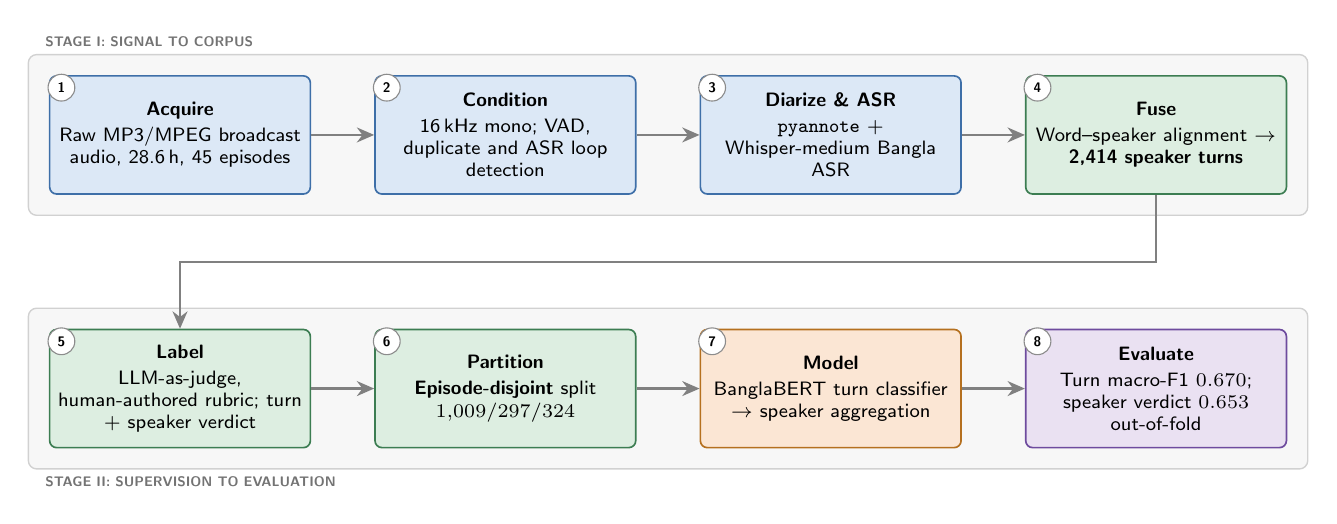
\begin{tikzpicture}[node distance=0mm]
\def\pw{31mm}
% ---- row 1: signal
\node[fbox=\pw, fill=cSig, draw=cSigB, minimum height=15mm] (b1)
  {\fhd{Acquire} Raw MP3/MPEG broadcast audio, 28.6\,h, 45 episodes};
\node[fbox=\pw, fill=cSig, draw=cSigB, minimum height=15mm, right=8mm of b1] (b2)
  {\fhd{Condition} 16\,kHz mono; VAD, duplicate and ASR loop detection};
\node[fbox=\pw, fill=cSig, draw=cSigB, minimum height=15mm, right=8mm of b2] (b3)
  {\fhd{Diarize \& ASR} \texttt{pyannote} $+$ Whisper-medium Bangla ASR};
\node[fbox=\pw, fill=cDat, draw=cDatB, minimum height=15mm, right=8mm of b3] (b4)
  {\fhd{Fuse} Word--speaker alignment $\rightarrow$ \textbf{2{,}414 speaker turns}};
% ---- row 2: supervision and modelling
\node[fbox=\pw, fill=cDat, draw=cDatB, minimum height=15mm, below=17mm of b1] (b5)
  {\fhd{Label} LLM-as-judge, human-authored rubric; turn $+$ speaker verdict};
\node[fbox=\pw, fill=cDat, draw=cDatB, minimum height=15mm, right=8mm of b5] (b6)
  {\fhd{Partition} \textbf{Episode-disjoint} split $1{,}009 / 297 / 324$};
\node[fbox=\pw, fill=cMod, draw=cModB, minimum height=15mm, right=8mm of b6] (b7)
  {\fhd{Model} BanglaBERT turn classifier $\rightarrow$ speaker aggregation};
\node[fbox=\pw, fill=cOut, draw=cOutB, minimum height=15mm, right=8mm of b7] (b8)
  {\fhd{Evaluate} Turn macro-F1 $0.670$; speaker verdict $0.653$ out-of-fold};
\foreach \i/\j in {b1/b2, b2/b3, b3/b4, b5/b6, b6/b7, b7/b8} \draw[farr] (\i) -- (\j);
% wrap from the end of row 1 to the start of row 2
\draw[farr] (b4.south) -- ++(0,-8.5mm) -| (b5.north);
\foreach \n/\k in {b1/1, b2/2, b3/3, b4/4, b5/5, b6/6, b7/7, b8/8}
  \node[fnum] at ($(\n.north west)+(1.6mm,-1.6mm)$) {\k};
\begin{scope}[on background layer]
  \node[band, fit=(b1)(b4), inner sep=2.6mm] (grow1) {};
  \node[band, fit=(b5)(b8), inner sep=2.6mm] (grow2) {};
\end{scope}
\node[bandlbl, anchor=north west] at ($(grow1.north west)+(1mm,3.4mm)$)
  {STAGE I: SIGNAL TO CORPUS};
\node[bandlbl, anchor=south west] at ($(grow2.south west)+(1mm,-3.4mm)$)
  {STAGE II: SUPERVISION TO EVALUATION};
\end{tikzpicture}
\end{center}

{\sffamily\small\setstretch{1.0}\textbf{Figure 2.} Technical pipeline followed in the course
project. Splitting is grouped by episode, never by row, so that turns from one panel cannot
appear on both sides of the split; the deduplicated episode is removed before partitioning. All
45 episodes carry trusted \texttt{pyannote} diarization in this build.\par}

\vspace{4pt}

\subsection{Data source and sampling strategy}

The source frame is publicly broadcast Bangla-language television programmes devoted to business
and economics. Each of the six group members independently collected five to six episodes into a
roll-numbered folder (\texttt{2107001}, \texttt{2107004}, \texttt{2107006}, \texttt{2107009},
\texttt{2107010}, \texttt{2107015}), giving 56 registry entries and 46 processed episodes.
Inclusion required a multi-speaker panel or interview format, a predominantly economic topic and
intelligible audio. Two exclusions were applied after profiling: one episode
(\texttt{2107010::ep006}) was found to be byte-identical in transcript content to
\texttt{2107004::ep006} and was removed by transcript hash, leaving \textbf{45 unique episodes};
and one episode (\texttt{2107015::ep002}) proved to be an interview on law and order rather than
economics, and is retained but flagged out-of-domain.

\subsection{Collection setting, period and location}

Episodes are studio-recorded broadcasts from Bangladeshi national channels, retrieved as
MP3/MPEG audio. Durations range from 1{,}411 s to 3{,}614 s (mean $\approx$2{,}420 s), totalling
approximately 17.5 hours. Pipeline execution took place on Google Colab (CUDA device) in
August 2026 with fixed seed 17; the speaker-sentiment stage was executed locally and on Colab
with seed 7.

\subsection{Instruments, hardware, software and versions}

\begin{tabularx}{\textwidth}{|L{3.4cm}|Y|}
\hline
\thd{Stage} & \thd{Component, version and settings} \\ \hline
Audio hygiene & Resample to 16 kHz mono WAV; loudness and clipping report written to
\texttt{processed/hygiene\_report.json} \\ \hline
Diarization & \texttt{pyannote/speaker-diarization-community-1}, revision
\texttt{3533c8cf8e369892e6b79ff1bf80f7b0286a54ee}, with
\texttt{wespeaker-voxceleb-resnet34-LM} embeddings; \texttt{min\_duration\_off} 0.1 s,
\texttt{min\_cluster\_size} 20, \texttt{min\_segment\_sec} 0.75,
\texttt{min\_speaker\_airtime\_sec} 9.0, \texttt{stitch\_gap\_sec} 2.0. Energy-based VAD fallback
when no Hugging Face token was present. \\ \hline
ASR & \texttt{bengaliAI/tugstugi\_bengaliai-asr\_whisper-medium}, revision
\texttt{da605cc1bd2f60a18d8e440e977ddfa921a88e63}, CTranslate2 runtime; \texttt{beam\_size} 5,
\texttt{repetition\_penalty} 0.8, \texttt{max\_chunk\_sec} 28.0; per-word probabilities retained \\ \hline
Fusion & Schema 2.0; word $\rightarrow$ speaker assignment
\texttt{midpoint\_then\_max\_overlap}; overlap policy \texttt{first-speaker-wins} \\ \hline
Labelling & Claude Opus 5 under a fixed rubric; structured JSON output schema \\ \hline
Modelling & \texttt{csebuetnlp/banglabert}, revision \texttt{9ce791f3}; PyTorch 2.12,
\texttt{transformers}, \texttt{scikit-learn}; hand-written training loop \\ \hline
\end{tabularx}

\subsection{Variables, measurements and metadata}

Per episode the registry records \texttt{episode\_id}, channel, programme title, duration (s),
sample rate, channels, codec, bit rate, file size, SHA-256 and a licence-attestation field. Per
word the fused files record start/end time (s), the token, an ASR probability, the assigned
\texttt{speaker\_id} and the assignment method. Per turn the corpus records the identifiers,
timing, text, word count, mean ASR confidence, diarization provider and trust flag, quality flags
and the inferred role. The complete field list is in Section 7.2 and Appendix A.

\subsection{Annotation / labeling protocol}

Labels were assigned by a Claude Opus 5 judge, one call per speaker--episode unit, returning the
speaker verdict \emph{and} every turn label in the same call so that turn labels are consistent
with the holistic verdict. All 150 eligible units were judged. The rubric encodes the failure modes of this genre:

\begin{itemize}[leftmargin=1.4em,itemsep=2pt,topsep=2pt]
  \item \textbf{Evaluative stance, not emotion.} A calm description of a banking collapse is negative.
  \item \textbf{Direction words are not polar.} ``Increased'' is positive for reserves and negative for inflation; polarity follows the orientation of the target.
  \item \textbf{A pointed question is neutral.} Hosts elicit, they do not assert.
  \item \textbf{A recommendation is neutral; a complaint is negative.}
  \item \textbf{Reported speech is not the speaker's own stance.}
  \item \texttt{illegible} is a first-class label for ASR-destroyed turns, which are then dropped from supervision rather than guessed.
\end{itemize}

Each turn label carries a confidence and an \textbf{evidence quote}. We measured how literal these
quotes are: \textbf{58\% occur verbatim in the turn they cite and 42\% are close paraphrases of it}
(59.4\% in the first judging round, 56.9\% in the second, so this is a stable property of the judge
rather than a regression). The quotes therefore localise a label to a specific turn and claim,
which is what makes manual spot-checking fast, but they are \emph{not} exact-match provenance
and must not be used as string keys. The measurement script is released with the corpus. \textbf{The shipped labels are a single judging pass}, produced in an
interactive session rather than through the batch API, so \texttt{pass\_agreement} equals 1.0 by
construction and no self-consistency figure exists yet. Multi-pass judging
(\texttt{--passes 3}) and the 180-turn human verification sample are specified in the repository
and are the designated next step (Sections 9 and 12).

\textbf{Re-judging after the second pipeline run.} When the bundles were re-processed, adding
twenty episodes and re-running \texttt{pyannote} over roll \texttt{2107009}, the turn
segmentation changed underneath most of the existing labels. A judgement was carried forward
\emph{only} if its speaker key still existed \emph{and} its ordered list of \texttt{turn\_id}s was
byte-identical to the rebuilt corpus. Fifty-three of the original judgements passed that test;
the remaining ninety-seven units were judged again from scratch against the new segmentation.
The merge script enforces the check programmatically and asserts a zero turn-count mismatch
across all 150 released blocks, so no label is silently attached to a turn it was not written
for.

\subsection{Human review and correction}

The labels are machine-authored but the corpus is not machine-accepted. Every stage between the
raw broadcast and the released supervision set passed through a human decision, and each of those
decisions left an artefact in the archive that a reader can check:

\begin{itemize}[leftmargin=1.4em,itemsep=3pt,topsep=2pt]
  \item \textbf{The rubric is human-written.} The six genre-specific rules above were written by
  the team after reading transcripts, not derived by the model. The judge's decisions are
  therefore constrained by human criteria that are published in full.
  \item \textbf{Diarization was audited and re-run.} Inspection of build~1 showed that roll
  \texttt{2107009} had been segmented by the fallback provider into unusable fragments;
  \texttt{ep001} alone produced 263 of them. The episode set for that roll was re-diarized with
  \texttt{pyannote} and \texttt{ep001} resolved to 47 real speaker turns. All 45 episodes in the
  released build carry \texttt{diarization\_trusted = true}; none did in build~1.
  \item \textbf{Units were screened before judging.} Of 212 reconstructed speaker units, 62 were
  rejected as unjudgeable and never sent, for untrusted diarization, an unassigned speaker, or
  fewer clean words than the human-set minimum, leaving 150. A further three were withdrawn from the
  speaker-level task after review, giving the 147 units carrying
  \texttt{speaker\_level\_valid = true}.
  \item \textbf{Out-of-domain material was caught by reading, not by a filter.} Two episodes were
  found on inspection to be off-genre (a law-and-order interview; a news bulletin spliced onto a
  talk show). Both are labelled \texttt{illegible} throughout so they contribute no supervision
  while remaining in the corpus for transparency.
  \item \textbf{Stale labels were detected and discarded, not repaired.} When the corpus was
  rebuilt, a judgement was carried forward only if its ordered \texttt{turn\_id} list was
  byte-identical to the new segmentation. Fifty-three passed; ninety-seven units were re-judged
  from scratch and nineteen stale blocks were dropped. The merge script asserts zero turn-count
  mismatch across all 150 released blocks.
  \item \textbf{ASR-destroyed turns are excluded rather than guessed.} 181 of the 1{,}811 turn
  labels are \texttt{illegible} and are dropped from supervision, leaving 1{,}630 supervised
  turns.
  \item \textbf{Evidence quotes were audited.} All 715 evidence quotes were checked against the
  turns they cite; 58\% are verbatim spans and 42\% close paraphrases. The measurement script ships
  with the corpus so the audit is repeatable.
\end{itemize}

\textbf{What this review does \emph{not} include, stated explicitly.} No independent human
annotator re-labelled individual turns. The per-episode annotation drafts in the roll folders
(\texttt{annotation\_drafts/}, 46 files, 5{,}395 utterances) were prepared for exactly that step
and every one of them still carries \texttt{human\_verified: false},
\texttt{annotation\_status: review\_required}, an empty \texttt{labels} list and an empty
\texttt{annotator\_id}. Human effort in this build went into deciding \emph{what was fit to
label} and \emph{what had to be thrown away}; it did not go into overruling the judge on
individual turns. Consequently every accuracy figure in this report is agreement with the judge,
not with human truth, and the 180-turn dual-annotated verification sample specified in
Section~12 remains the first item of future work.

\subsection{Provenance, versioning and raw-data preservation}

Raw audio is preserved unmodified in the roll folders and is never overwritten; all derived
artefacts are written to a separate \texttt{results/} tree per roll. A \texttt{run\_manifest.json}
records the full configuration and a SHA-256 for every produced file, and a
\texttt{models/manifest.json} records the model URI, commit hash and notes for each network used.
Identifiers are hierarchical and stable: \texttt{roll::episode::turnNNNN}, with
\texttt{global\_episode} = \texttt{roll::episode} used as the grouping key for splitting.

%=======================================================================
\section{Data Description / Data Records}
%=======================================================================

\emph{\small Explain exactly what a user will find in the released dataset. The folder/file
structure should be understandable without opening every file. Include raw and processed
components separately.}

\subsection{A worked example: one moment of audio, end to end}

Before the file listings, Figure~\ref{fig:sample} follows a single moment of one episode through every stage of
the release, so that a reader can see what the data actually contains rather than only how it is
filed. Nothing in the figure is retyped: \texttt{make\_sample\_figure.py} reads it straight out
of the released files, so it cannot drift from the corpus.

% Figures 1 and 2 are hand-numbered TikZ drawings, so the float counter has to
% start after them or the captions would restart at 1.
\setcounter{figure}{2}

\begin{figure}[htbp]\centering
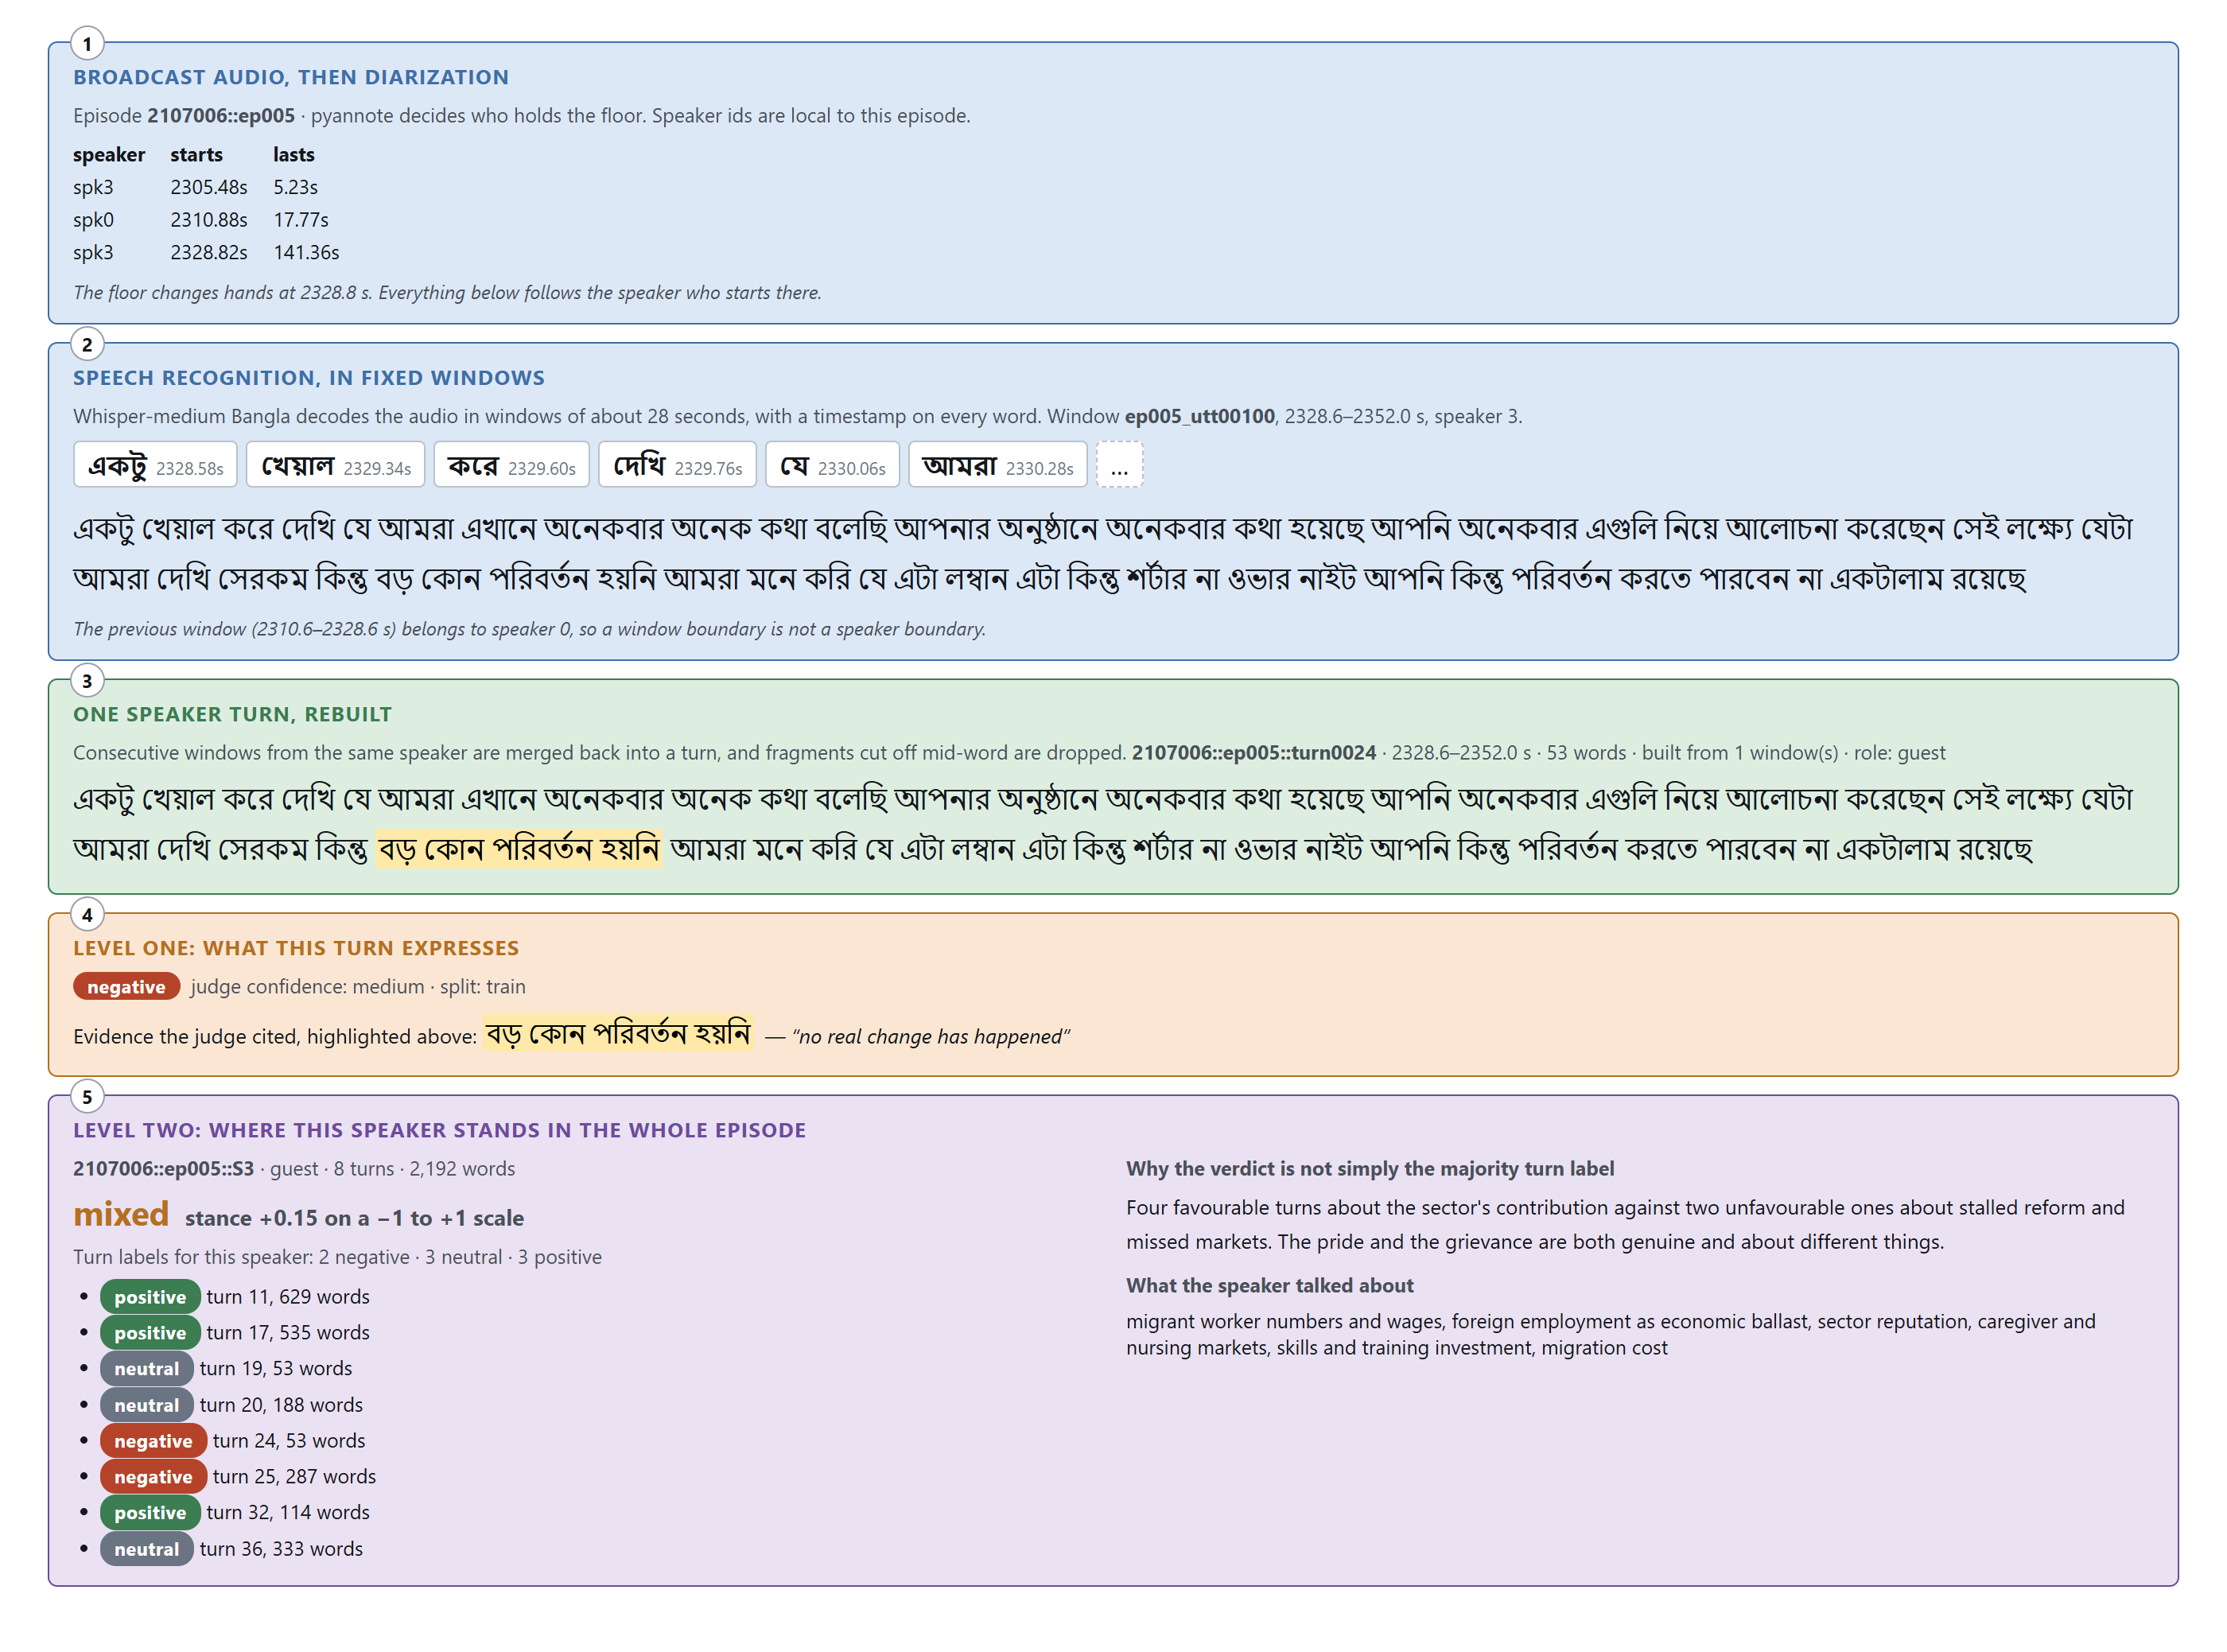
\includegraphics[width=\textwidth]{figs/dataset_sample.png}
\caption{One moment of \texttt{2107006::ep005}, from audio to speaker verdict. Diarization hands
the floor to speaker~3 at 2328.8\,s; Whisper decodes the next window with a timestamp on every
word; the window is merged back into a speaker turn; the judge labels that turn
\texttt{negative} and cites the span highlighted in the text; and the speaker's verdict for the
whole episode is \texttt{mixed}. The last two disagree on purpose. This guest is favourable about
what migrant labour contributes and unfavourable about stalled reform, and the release records
both levels rather than forcing one of them.}\label{fig:sample}
\end{figure}

\vspace{2pt}
Three properties of the corpus are visible in that single figure. A decode-window boundary is not
a speaker boundary, which is why the windows are merged back into turns before anything is
labelled. Turn labels carry a cited span, so a reader can check a label against the text without
listening to the audio. And the speaker verdict is a separate judgement, not a tally of the turn
labels beneath it.

\subsection{Repository / Folder Structure}

\begingroup\footnotesize
\begin{longtable}{|L{4.5cm}|L{7.4cm}|L{2.4cm}|}
\hline
\thd{Folder / file} & \thd{Contents} & \thd{Raw / processed / metadata} \\ \hline
\endfirsthead
\hline \thd{Folder / file} & \thd{Contents} & \thd{Raw / processed / metadata} \\ \hline \endhead
\texttt{<roll>/*.mp3, *.mpeg}          & Source broadcast audio as collected (not redistributed) & Raw \\ \hline
\texttt{<roll>/results/}\newline\texttt{raw/}           & \texttt{registry.csv}, \texttt{episode\_metadata.csv}: per-episode provenance and checksums & Metadata \\ \hline
\texttt{<roll>/results/}\newline\texttt{processed/}     & 16 kHz mono WAV per episode;\newline \texttt{hygiene\_report.json} & Processed \\ \hline
\texttt{<roll>/results/}\newline\texttt{diarization/}   & \texttt{epNNN.json}, \texttt{epNNN.rttm},\newline \texttt{epNNN\_raw.rttm}: speaker segments & Processed \\ \hline
\texttt{<roll>/results/}\newline\texttt{asr/}           & \texttt{epNNN.json}: transcripts with per-word timings and probabilities & Processed \\ \hline
\texttt{<roll>/results/}\newline\texttt{fused/}         & \texttt{epNNN.json}: word $\rightarrow$ speaker aligned utterances (schema 2.0) & Processed \\ \hline
\texttt{<roll>/results/}\newline\texttt{drafts/}, \texttt{annotated/} & Annotation drafts and review status & Metadata \\ \hline
\texttt{<roll>/results/}\newline\texttt{aggregated/}    & \texttt{submission\_gates.json}\newline automated quality gates & Metadata \\ \hline
\texttt{<roll>/results/}\newline\texttt{artifacts/},\newline \texttt{models/} & \texttt{run\_manifest.json},\newline \texttt{manifest.json}: config, checksums, model provenance & Metadata \\ \hline
\texttt{speaker\_sentiment/}\newline\texttt{data/} & \texttt{turns.jsonl}, \texttt{speakers.jsonl}, \texttt{judgements.jsonl}, \texttt{turns\_labelled.jsonl}, \texttt{speakers\_labelled.jsonl}, \texttt{turns\_\{train,val,test\}.jsonl}, \texttt{speakers\_\{train,val,test\}.jsonl} & Processed / ML-ready \\ \hline
\texttt{speaker\_sentiment/}\newline\texttt{*.py} & \texttt{build\_speaker\_corpus.py}, \texttt{llm\_judge.py}, \texttt{make\_datasets.py}, \texttt{predict\_speakers.py} & Code \\ \hline
\texttt{speaker\_sentiment/}\newline\texttt{*.ipynb} & \texttt{Speaker\_Sentiment\_BanglaBERT.ipynb}: training, aggregation, ablation, verification & Code \\ \hline
\texttt{speaker\_sentiment/}\newline\texttt{runs/} & Trained model, \texttt{metrics.json}, \texttt{test\_predictions.jsonl} & Results \\ \hline
\texttt{sentiment/lexicon/}            & \texttt{financial\_targets.csv} (52 targets), \texttt{polarity\_cues.csv} (103 cues) & Metadata \\ \hline
\texttt{README.md}                     & Access, pipeline, caveats and run instructions & Documentation \\ \hline
\end{longtable}
% This longtable has no caption, so it must not consume a table number.
\addtocounter{table}{-1}
\endgroup

\subsection{Data Dictionary}

Representative fields of \texttt{turns.jsonl}, the primary release file. The complete dictionary
for all release files is in Appendix~A.

\begingroup\footnotesize
\begin{longtable}{|L{2.6cm}|L{3.5cm}|L{1.6cm}|L{2.1cm}|L{2.8cm}|L{1.9cm}|}
\hline
\thd{Variable} & \thd{Meaning} & \thd{Type} & \thd{Unit / range} & \thd{Allowed values} & \thd{Missing rule} \\ \hline
\endfirsthead
\hline \thd{Variable} & \thd{Meaning} & \thd{Type} & \thd{Unit / range} & \thd{Allowed values} & \thd{Missing rule} \\ \hline \endhead
\texttt{turn\_id}      & Unique turn identifier & string & n/a & \texttt{roll::ep::}\newline\texttt{turnNNNN} & never null \\ \hline
\texttt{global\_episode} & Episode grouping key used for splitting & string & n/a & \texttt{roll::epNNN} & never null \\ \hline
\texttt{speaker\_id}   & Diarization cluster index within the episode & integer & $\ge -1$ & $-1$ = unassigned & $-1$ \\ \hline
\texttt{start\_sec}, \texttt{end\_sec} & Turn boundaries in the episode & float & seconds & $\ge 0$ & never null \\ \hline
\texttt{text}          & Normalised Bangla transcript of the turn & string & n/a & free text & \texttt{""} if empty \\ \hline
\texttt{n\_words}      & Whitespace word count of \texttt{text} & integer & $\ge 0$ & n/a & never null \\ \hline
\texttt{asr\_confidence} & Mean log-probability over the turn's words & float & $\le 0$ & n/a & null if no words \\ \hline
\texttt{diarization\_trusted} & False for the five fallback-diarized episodes & boolean & n/a & \texttt{true}/\texttt{false} & never null \\ \hline
\texttt{role}          & Inferred conversational role & string & n/a & \texttt{host}, \texttt{guest}, \texttt{minor}, \texttt{unassigned} & \texttt{unassigned} \\ \hline
\texttt{label}         & Judge turn label (labelled files only) & string & n/a & \texttt{negative}, \texttt{neutral}, \texttt{positive} & row dropped if \texttt{illegible} \\ \hline
\texttt{judge\_confidence} & Judge's stated confidence in the turn label & float & $[0,1]$ & n/a & never null \\ \hline
\texttt{evidence}      & Verbatim quote supporting the label & string & n/a & substring of \texttt{text} & \texttt{""} \\ \hline
\end{longtable}
% This longtable has no caption, so it must not consume a table number.
\addtocounter{table}{-1}
\endgroup

\emph{\small If the dataset has many variables, keep only representative rows here and place the
complete data dictionary in Appendix A and/or the repository.}

\subsection{Dataset Composition and Descriptive Overview}

\emph{\small Provide concise descriptive information needed to understand dataset composition:
counts by class/category, number of subjects/sources, temporal/geographic coverage, missingness
summary, and representative examples. Do not turn this into a full research-results section.}

\begin{tabularx}{\textwidth}{|L{6.6cm}|Y|}
\hline
\thd{Property} & \thd{Value} \\ \hline
Unique episodes (after transcript-hash dedup) & 45 (from 46 processed, 56 registry rows) \\ \hline
Episodes with trusted (\texttt{pyannote}) diarization & \textbf{45, all of them} \\ \hline
Episodes with fallback diarization & 0 (was 5 in build 1; re-diarized) \\ \hline
Total audio & $\approx$28.6 h \\ \hline
ASR decode windows & 5{,}327 \\ \hline
Speaker turns & \textbf{2{,}414} ($\approx$219{,}000 words) \\ \hline
Turns by role & guest 1{,}236, host 926, unassigned 233, minor 19 \\ \hline
Speaker--episode units & 212 total; 150 judged; 147 speaker-level valid (45 hosts, 103 guests, 2 minor) \\ \hline
Turn labels produced & 1{,}811; \texttt{illegible} 181 (10.0\%) dropped \\ \hline
Supervised turns & \textbf{1{,}630}: negative 53.4\%, neutral 34.7\%, positive 11.9\% \\ \hline
Speaker verdicts & negative 110, neutral 18, positive 11, mixed 8 \\ \hline
Human sentiment labels & \textbf{0} (see Sections 9 and 12) \\ \hline
\end{tabularx}

\vspace{4pt}
Role structure separates cleanly and confirms the rubric behaved as designed: hosts take many
short turns (mean 39 words) and are majority \texttt{neutral}, while guests take few long turns
(mean 146 words) and carry the evaluative content. Table~\ref{tab:roledist} gives the breakdown.

\begin{table}[htbp]\centering
\caption{Turn-label distribution by inferred speaker role over the 1{,}630 supervised turns.
Host neutrality is the expected consequence of the rubric rule that a pointed question is
elicitation rather than assertion. The pattern held after the corpus grew by 22\%, which is
evidence the rubric was applied consistently across both judging rounds.}\label{tab:roledist}
\begin{tabular}{|l|r|r|r|r|}
\hline
\thd{Role} & \thd{Negative} & \thd{Neutral} & \thd{Positive} & \thd{Total} \\ \hline
Guest      & 602 & 192 & 171 & 965 \\ \hline
Host       & 266 & 374 & 23  & 663 \\ \hline
Minor      & 2   & 0   & 0   & 2 \\ \hline
\textbf{Total} & \textbf{870} & \textbf{566} & \textbf{194} & \textbf{1{,}630} \\ \hline
\end{tabular}
\end{table}

%=======================================================================
\section{Data Preprocessing, Curation and Leakage Control}
%=======================================================================

\emph{\small Document every transformation from raw data to the released/ML-ready data. Preserve
the distinction between data cleaning and model-specific preprocessing.}

\begin{itemize}[leftmargin=1.4em,itemsep=3pt,topsep=2pt]
  \item \textbf{Cleaning.} One duplicate episode was removed by transcript hash. Repetition-loop
        turns, an ASR failure mode in which one syllable repeats for hundreds of characters,
        are detected and flagged \texttt{flag\_repetition\_loop}. Turns below a minimum length are
        flagged \texttt{flag\_too\_short}.
  \item \textbf{Window $\rightarrow$ turn reconstruction.} The ``utterances'' in the fused files
        are \emph{not} turns: they are fixed $\approx$28 s ASR decode windows, a large fraction of
        the 5{,}327 having a duration of 27.2--28.0 s. Every window boundary truncates a word, so
        many windows begin with an orthographically impossible Bengali dependent sign. Consecutive
        same-speaker windows are therefore merged back into turns and orphaned fragments dropped.
  \item \textbf{Missing data.} Words that fusion could not attribute carry
        \texttt{speaker\_id = -1}; the corresponding turns are retained with
        \texttt{role = unassigned} and a \texttt{diarization\_trusted} flag, rather than deleted or
        imputed. Missingness is flagged, never silently filled.
  \item \textbf{Outliers / noise.} Turns the judge marked \texttt{illegible} (181, 10.0\%) are
        retained in \texttt{turns.jsonl} but excluded from \texttt{turns\_labelled.jsonl} and all
        splits, so the raw record is preserved while supervision stays clean.
  \item \textbf{Encoding / normalisation (model-specific).} Unicode NFC normalisation, with the
        \texttt{csebuetnlp} normalizer applied where available because BanglaBERT was pretrained
        on normalised text. Inputs are constructed as \texttt{role\_turn} sentence pairs and
        tokenised at \texttt{max\_len} 128 on CPU or 256 on GPU; 256 truncates $\approx$10\% of
        turns and 128 truncates $\approx$23\% (subword length p50 = 46, p75 = 120, p90 = 254,
        p95 = 351, max = 1{,}265).
  \item \textbf{Augmentation / synthetic data.} None. No synthetic turns or oversampled copies were
        created; class imbalance is handled by class weighting in the loss, not by resampling.
  \item \textbf{De-identification.} Speakers are released as episode-local cluster indices
        (\texttt{Speaker 0}, \texttt{Speaker 1}, \dots) and are never linked to named individuals.
        Speaker IDs are model predictions, not person identities.
  \item \textbf{Leakage control.} The grouping key is \texttt{global\_episode}. Splits are
        constructed episode-disjointly and \texttt{make\_datasets.py} \emph{asserts} disjointness
        rather than assuming it, because two turns from one talk show share the panel, the topic,
        the presenter's phrasing and the same ASR error signature, so a random row split would let
        the model recognise the episode instead of the stance. The duplicate episode was removed
        \emph{before} splitting, so the same panel cannot appear on both sides.
        \textbf{Known residual risk:} a programme-level split is the stricter control, but a
        majority of episodes carry a placeholder or empty programme title in the registry, so
        grouping by programme collapses the corpus; the split therefore warns that train and test share the programme
        label \texttt{business talk}, and this is accepted knowingly (Section 12).
\end{itemize}

%=======================================================================
\section{Technical Validation and Data Quality}
%=======================================================================

\emph{\small This section supports the technical quality of the dataset. Validation should concern
the data, not merely model accuracy.}

\begin{longtable}{|L{3.6cm}|L{11.8cm}|}
\hline
\thd{Quality dimension} & \thd{Evidence / checks performed} \\ \hline
\endfirsthead
\hline \thd{Quality dimension} & \thd{Evidence / checks performed} \\ \hline \endhead
\thd{Completeness}   & 56 registry rows $\rightarrow$ 46 processed episodes $\rightarrow$ 45 unique. Every retained episode has diarization, ASR, fusion and draft artefacts; per-episode counts are reconciled in the \texttt{stats} block of each fused file. Automated gates in \texttt{submission\_gates.json} record which checks pass, fail or are skipped. \\ \hline
\thd{Consistency}    & Fused files validate against schema 2.0. Turn counts, word counts and durations are recomputed from the fused files at corpus-build time and cross-checked. Identifier format is enforced; episode disjointness across splits is asserted programmatically. \\ \hline
\thd{Label quality}  & Single-pass LLM judge with a fixed, byte-identical rubric and structured JSON output. Every turn label carries a confidence and an evidence quote; 58\% of the 715 quotes are verbatim spans of the cited turn and 42\% are close paraphrases (measured, both rounds alike), so labels are spot-checkable but the quotes are not exact provenance. \textbf{Internal coherence measured:} rebuilding each speaker verdict bottom-up from its own turn labels, without showing the aggregator the holistic verdict, reproduces it 85.0\% of the time exactly (\texttt{word\_weighted}) and 87.1\% by polar direction (\texttt{majority\_vote}). Coherence \emph{rose} from 78.7\%/83.6\% when the corpus grew from 72 to 150 judged units, which is evidence of a stable rubric rather than drift. \textbf{Not yet measured:} inter-pass self-consistency (labels are one pass) and agreement with human annotators. \\ \hline
\thd{Measurement quality} & Fixed decoding settings (beam 5, repetition penalty 0.8, 28 s chunks) and fixed diarization thresholds across all episodes. Per-word ASR probabilities and per-turn mean confidence are retained so low-confidence material can be filtered downstream. Audio hygiene reports are stored per episode. \\ \hline
\thd{Integrity}      & SHA-256 recorded for every source file in \texttt{registry.csv} and for every produced file in \texttt{run\_manifest.json}; \texttt{sha256\_verified} is true for all registry rows. Exact-duplicate detection is by transcript hash. \\ \hline
\thd{Representativeness / bias} & Class imbalance persists (positive is 11.9\% of supervised turns, up from 10.2\%). Strong negative prior (110 of 150 speaker verdicts). This is \emph{partly real}, since the episodes cover a banking crisis, a reserve crisis, an energy shock and inflation, and \emph{partly selection and possible judge drift}; the two explanations are separated only by human verification. Diarization is now uniform: all 45 episodes are \texttt{pyannote}. Two episodes contain out-of-domain material (one law-and-order interview; one news bulletin spliced onto a talk show), and both are labelled \texttt{illegible} throughout so they never enter supervision. \\ \hline
\thd{Reproducibility} & \texttt{build\_speaker\_corpus.py} regenerates \texttt{turns.jsonl} and \texttt{speakers.jsonl} from the fused bundles in $\approx$20 s; \texttt{make\_datasets.py} regenerates all six split files in $\approx$5 s with an explicit seed (13). Pipeline seed 17 and every model revision hash are recorded in \texttt{run\_manifest.json}. The baseline trains on CPU in $\approx$60 min, so results are re-derivable without a GPU. \\ \hline
\end{longtable}
% This longtable has no caption, so it must not consume a table number.
\addtocounter{table}{-1}

\vspace{2pt}
\textbf{Gates that remain open, reported honestly.} \texttt{submission\_gates.json} records
\texttt{wer\_measured}, \texttt{der\_measured} and \texttt{annotation\_kappa} as
\texttt{SKIPPED} because no gold transcript, gold RTTM or second annotation file exists.
Every number in Section 10 is therefore bounded by an unmeasured word error rate.

\subsection{Comparison with Existing Datasets and Significance}

\emph{\small Compare the dataset with similar, related and competitive datasets with proper
citation in tabular form.}

\vspace{2pt}
Four properties decide whether a resource can answer the question in Figure~1. It has to be
\textbf{Bangla}; it has to be \textbf{spoken} material rather than writing; it has to keep
\textbf{who said what} instead of pooling a conversation into one text; and it has to carry a
\textbf{verdict on the person}, not only on each sentence. The table below scores the nearest resources
on those four. Each is strong on some and silent on others; the gap this dataset fills is the
row where all four are present at once.

\begin{longtable}{|L{3.0cm}|L{1.5cm}|L{1.3cm}|L{1.6cm}|L{1.7cm}|L{4.4cm}|}
\hline
\thd{Dataset} & \thd{Bangla} & \thd{Spoken} & \thd{Speaker kept apart} & \thd{Verdict on the person} & \thd{What it gives, and what it cannot} \\ \hline
\endfirsthead
\hline \thd{Dataset} & \thd{Bangla} & \thd{Spoken} & \thd{Speaker} & \thd{Person verdict} & \thd{Relation} \\ \hline \endhead
BLUB / BanglaBERT \cite{banglabert} & Yes & No & No & No & Supplies the encoder this work fine-tunes. Written text, one label per document. \\ \hline
BLP-2023 Task 2 \cite{blp2023} & Yes & No & No & No & The closest Bangla sentiment benchmark. Social-media posts have a single author and no floor to share. \\ \hline
BAN-ABSA \cite{banabsa} / BABSA \cite{babsa} & Yes & No & No & No & Ties sentiment to a target, which this work also needs, but the target is an aspect in written text, never a participant in a conversation. \\ \hline
MELD / IEMOCAP \cite{erc} & No & Yes & Yes & No & Proves conversational, speaker-aware labelling works. English, scripted or acted, and the label stops at the utterance. \\ \hline
Earnings-call corpora \cite{earnings} & No & Yes & Yes & Partly & Nearest in intent: financial speech attributed to named executives. English, professionally transcribed, so it never tests robustness to ASR error. \\ \hline
\textbf{This dataset} & \textbf{Yes} & \textbf{Yes} & \textbf{Yes} & \textbf{Yes} & \textbf{Bangla broadcast debate, ASR-noisy, 2{,}414 turns kept per speaker, 147 speaker--episode verdicts with a stance score.} \\ \hline
\end{longtable}
% This longtable has no caption, so it must not consume a table number.
\addtocounter{table}{-1}

\vspace{2pt}
\textbf{The distinction in one sentence.} Every Bangla sentiment resource we could find labels
writing, and every speaker-aware conversational resource we could find is in English and stops at
the utterance; this dataset is the intersection, and it adds the level neither side has, which is
a verdict on a participant across a whole episode.

\emph{\small Identify and mention in points the novelty and significant properties of the dataset
w.r.t.\ existing datasets.}

\begin{itemize}[leftmargin=1.4em,itemsep=2pt,topsep=2pt]
  \item \textbf{Two supervised tasks, not one.} The release supports turn sentiment (1{,}630
        labelled turns) and a separate verdict on each speaker across a whole episode (147 units
        with a stance score). Both are given a full evaluation in Section 10, with baselines,
        confusion matrices and slice breakdowns for each.
  \item \textbf{The second task is measurably not reducible to the first.} Both levels come from
        one judging call over the speaker's full script, so they are coherent by construction, and
        rebuilding the verdict from its own turn labels reproduces it 85.0\% of the time. The
        remaining 15\% is the point: an oracle holding the gold turn labels still cannot recover
        those verdicts, so roughly one speaker in seven can only be judged from the episode. That
        is the headroom a speaker-level model exists to capture, and no utterance-level corpus
        exposes it.
  \item \textbf{Speaker--episode as a released unit.} Existing conversational sentiment corpora stop
        at the utterance; this release ships the speaker unit with a continuous stance
        score, which is the unit financial analysis actually needs.
  \item \textbf{First Bangla speaker-attributed sentiment resource in broadcast financial speech},
        to the best of our search; the existing Bangla resources are written text.
  \item \textbf{Genre-specific rubric.} The host-question-is-neutral and target-orientation rules
        are specific to panel discussion and to economic vocabulary, and the role split in the
        released labels demonstrates they took effect.
  \item \textbf{Full intermediate provenance.} RTTM, per-word ASR probabilities, fusion alignments
        and judge rationales are all retained, so the corpus can be re-derived under a different
        diarizer, ASR model or labelling rule.
  \item \textbf{Documented defects, and a documented repair.} The duplicate episode, the
        out-of-domain material and the placeholder programme titles are published rather than
        concealed. Two defects reported in build 1 have since been fixed: roll \texttt{2107009}
        was re-diarized with \texttt{pyannote}, and the degenerate speaker-level validation split
        (six units over two classes) now holds 23 units over all four classes.
\end{itemize}

%=======================================================================
\section{Machine Learning (ML) Use Demonstration}
%=======================================================================

\emph{\small The purpose is to demonstrate that the dataset can support a valid ML workflow. Keep
the emphasis on dataset usability and reproducibility rather than claiming a new algorithm.}

\subsection{ML task definition}

The dataset defines \textbf{two tasks, not one}, and they are evaluated separately because they
are different problems.

\vspace{2pt}
\textbf{Task A, turn sentiment.} Input $X$ is the pair (\texttt{role}, \texttt{turn text}); the
target $y \in$ \{\texttt{negative}, \texttt{neutral}, \texttt{positive}\}; the unit of prediction
is one speaker turn. There are 1{,}630 supervised turns.

\vspace{2pt}
\textbf{Task B, the speaker's position across the whole episode.} Input is everything one speaker
said in one episode; the target $y \in$ \{\texttt{negative}, \texttt{mixed}, \texttt{neutral},
\texttt{positive}\} together with a continuous stance score in $[-1, 1]$; the unit of prediction
is one speaker--episode unit. There are 147 such units.

\vspace{2pt}
\textbf{Why Task B is not Task A with a summing step.} A verdict on a person is not the average of
their sentences. A panellist can concede a point warmly and still hold a negative position; a
host can sound severe while taking no position at all; and the \texttt{mixed} verdict has no
turn-level counterpart, because it describes a speaker who is genuinely favourable about one
thing and unfavourable about another. Figure~\ref{fig:sample} shows a real case from the release: a guest whose
eight turns are three positive, three neutral and two negative, and whose episode verdict is
\texttt{mixed} with a stance of $+0.15$. The Task B results below quantify the gap. Even an oracle that is
handed the judge's own gold turn labels and combines them perfectly recovers only 85.0\% of the
speaker verdicts, so roughly one verdict in seven is not present in the turn labels at all and
has to be read from the episode. Task A therefore cannot subsume Task B, and the report measures
both.

\subsection{Data partitioning strategy}

Episode-grouped split, \textbf{never} a row split, with seed 13 and the configuration
\texttt{--group-by episode --test-episodes 9 --val-episodes 7}. Seven candidate seeds were
compared on class balance before one was fixed; seed 13 is the only one placing all four speaker
classes and a workable share of positive turns in every partition. Table~\ref{tab:partition} gives the partition.

\begin{table}[htbp]\centering
\caption{Episode-disjoint partition of the supervised corpus (seed 13). All three splits carry
all three turn classes and all four speaker classes; the degenerate validation split reported in
build 1 no longer occurs.}\label{tab:partition}
\begin{tabular}{|l|r|r|r|r|r|r|}
\hline
\thd{Split} & \thd{Episodes} & \thd{Speakers} & \thd{Turns} & \thd{Neg.} & \thd{Neu.} & \thd{Pos.} \\ \hline
Train & 29 & 94 & 1{,}009 & 530 & 365 & 114 \\ \hline
Val   & 7  & 23 & 297     & 162 & 93  & 42 \\ \hline
Test  & 9  & 30 & 324     & 178 & 108 & 38 \\ \hline
\end{tabular}
\end{table}

Leakage rationale: turns from one episode share the panel, topic, presenter phrasing and ASR
error signature. Disjointness is asserted in code. The duplicated episode was removed before
splitting. Speaker-level, the partition holds 94 / 23 / 30 valid units; the validation split now
contains negative 16, neutral 3, positive 2 and mixed 2, so speaker-level validation is
meaningful for the first time.

\subsection{Preprocessing and feature/representation steps}

Unicode NFC plus the \texttt{csebuetnlp} normalizer; \texttt{role\_turn} sentence-pair
construction; BanglaBERT WordPiece tokenisation at \texttt{max\_len} 128 (CPU run) or 256 (GPU). No vocabulary, scaler or
statistic is fitted on validation or test data: the tokenizer is pretrained and the class
weights are computed on the training split only.

\subsection{ML model(s) and hyperparameters}

\begin{tabularx}{\textwidth}{|L{4.0cm}|Y|}
\hline
\thd{Majority-class baseline} & Predicts the most frequent training class; reported as the floor. \\ \hline
\thd{TF--IDF + logistic regression} & Word 1--2-grams (\texttt{min\_df}=2, sublinear TF), balanced class weights. The feature family (word 1--2, \texttt{char\_wb} 2--5, \texttt{char\_wb} 3--5) and $C\in\{0.5,1,2,4,8\}$ were selected together on the validation split; word 1--2 with $C=2$ won at 0.578. Reproducible with \texttt{tfidf\_baseline.py}. \\ \hline
\thd{BanglaBERT (main)} & \texttt{csebuetnlp/banglabert} (ELECTRA discriminator, 110M), \texttt{input\_mode = role\_turn}, \texttt{max\_len} 256, 6 epochs (best epoch 4, restored by validation macro-F1), batch 16, AdamW with encoder LR $2\times10^{-5}$ and head LR $1\times10^{-4}$, linear warmup 10\%, weight decay 0.01, gradient clipping 1.0, label smoothing 0.1, class weighting \textbf{on} (positive is 11.9\% of the data), per-sample weights from judge confidence $\times$ pass agreement, seed 42. Trained on a Colab T4. Hand-written training loop rather than \texttt{Trainer}, so the two weighting schemes compose cleanly. \\ \hline
\end{tabularx}

\subsection{Evaluation metrics}

\textbf{Macro-F1} is the headline metric because the corpus is strongly imbalanced and the
positive class, the one a financial sentiment index most needs, is the rarest. Reported
alongside: per-class precision/recall, the majority-class macro-F1 floor, and, at the speaker
level, exact verdict accuracy, polar-direction accuracy, and Pearson correlation between the
predicted and judged stance scores.

\subsection{Reproducibility}

Notebook \texttt{speaker\_sentiment/Speaker\_Sentiment\_BanglaBERT.ipynb}; corpus rebuilt by
\texttt{build\_speaker\_corpus.py} and \texttt{make\_datasets.py}; CLI scoring by
\texttt{predict\_speakers.py}, which reads \texttt{input\_mode}, \texttt{max\_len} and the winning
aggregation rule out of the written \texttt{metrics.json} so the CLI cannot silently disagree with
the model that produced it. Split seed 13, training seed 42. The reported run was executed on a
Colab T4 GPU; \texttt{history.csv}, \texttt{metrics.json}, \texttt{test\_predictions.jsonl} and the
\texttt{presentation/} artefacts in \texttt{runs/banglabert\_turn/} are released so every figure and
table below can be recomputed without retraining. Measured runtime: $\approx$30 min for 6 epochs at
\texttt{max\_len} 128 on CPU (10 threads), $\approx$60 min at 256; $\approx$3 min on a Colab T4.
On Windows, \texttt{python -X utf8} is required.

\subsection{Results (compact)}

\begin{table}[htbp]\centering
\caption{Turn-level results on the episode-disjoint test split (324 turns). Macro-F1 is the
headline metric because the positive class is only 11.9\% of the supervised corpus. Both learned
models were selected on the validation split and evaluated once on test.}
\begin{tabular}{|l|c|c|c|c|L{3.1cm}|}
\hline
\thd{Model} & \thd{Val macro-F1} & \thd{Test macro-F1} & \thd{Test acc.} & \thd{$\kappa$} & \thd{Notes} \\ \hline
Majority class            & n/a    & 0.236 & 0.549 & 0.000 & Floor \\ \hline
TF--IDF word 1--2 + LogReg & 0.578 & 0.529 & 0.623 & 0.339 & Non-neural reference; $C=2$ \\ \hline
\textbf{BanglaBERT (\texttt{role\_turn})} & \textbf{0.704} & \textbf{0.670} & \textbf{0.701} & \textbf{0.496} & Main baseline; class-weighted \\ \hline
\end{tabular}
\end{table}

\begin{table}[htbp]\centering
\caption{Per-class turn-level performance of the BanglaBERT baseline on the test split.
The rarest class, \texttt{positive}, is the weakest but remains far above chance; the
class-weighted loss is what keeps its recall usable.}
\begin{tabular}{|l|c|c|c|r|}
\hline
\thd{Class} & \thd{Precision} & \thd{Recall} & \thd{F1} & \thd{Support} \\ \hline
\texttt{negative} & 0.790 & 0.697 & 0.740 & 178 \\ \hline
\texttt{neutral}  & 0.655 & 0.722 & 0.687 & 108 \\ \hline
\texttt{positive} & 0.521 & 0.658 & 0.581 & 38 \\ \hline
\textbf{Macro avg} & \textbf{0.655} & \textbf{0.692} & \textbf{0.670} & \textbf{324} \\ \hline
Weighted avg & 0.713 & 0.701 & 0.704 & 324 \\ \hline
\end{tabular}
\end{table}

\begin{figure}[htbp]\centering
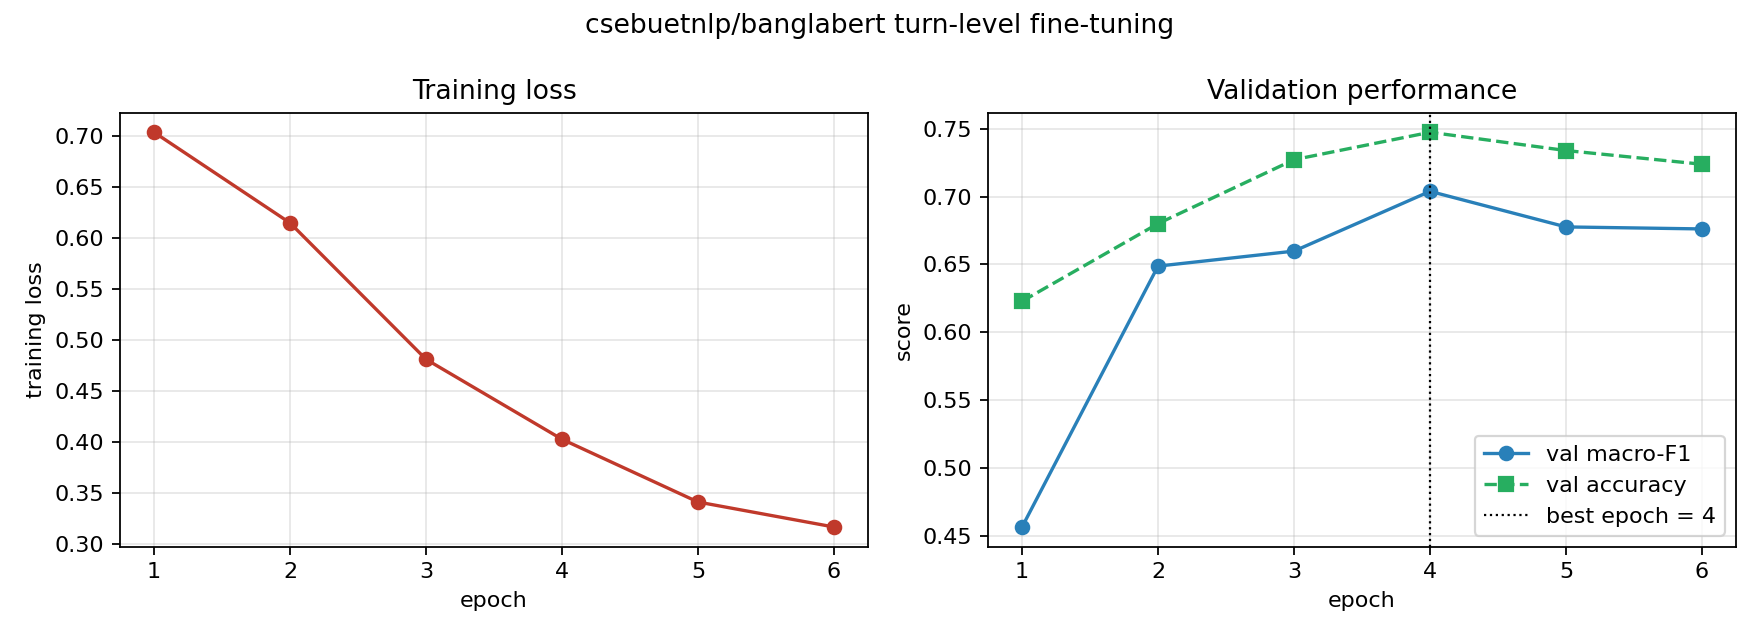
\includegraphics[width=\textwidth]{figs/training_curves.png}
\caption{Training loss and validation performance per epoch. Validation macro-F1 peaks at epoch 4
(0.704) and then declines while training loss keeps falling. The model begins to overfit the
1{,}009 training turns, and the epoch-4 checkpoint is the one restored and evaluated.}
\end{figure}

\begin{figure}[htbp]\centering
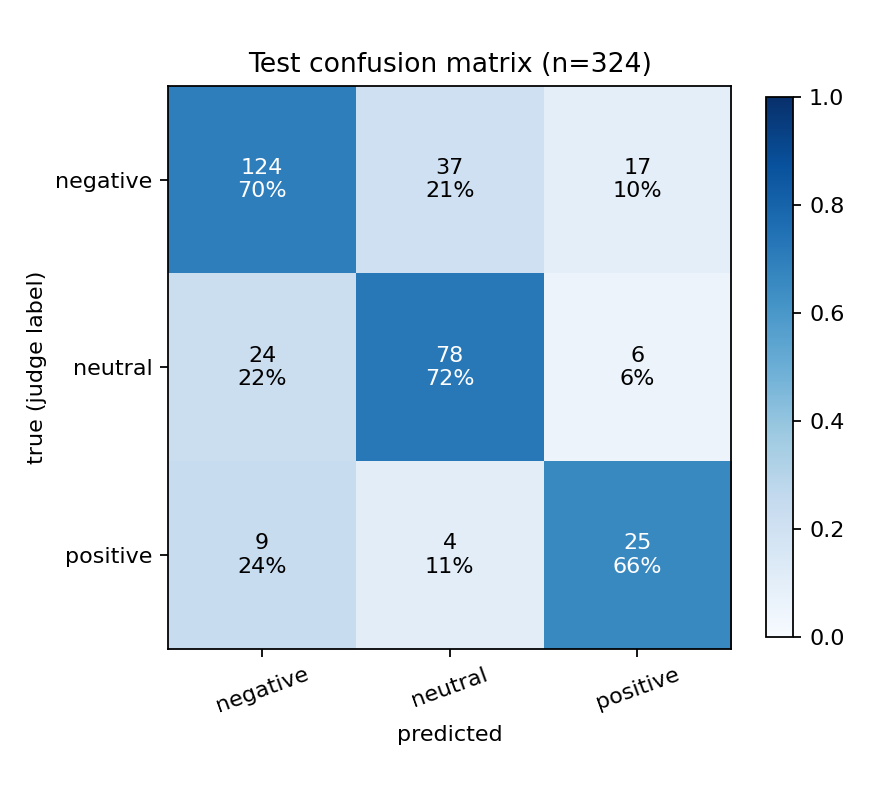
\includegraphics[width=0.62\textwidth]{figs/confusion_matrix.png}
\caption{Test confusion matrix (counts and row-normalised). The dominant error is
\texttt{negative} misread as \texttt{neutral} (37 turns): understated criticism in a panel
register, which is exactly the distinction the rubric was written to enforce.}
\end{figure}

\vspace{2pt}
\textbf{Where the errors are.} Of 97 test errors, 37 are \texttt{negative} turns predicted
\texttt{neutral} and 24 are \texttt{neutral} predicted \texttt{negative}; the
\texttt{positive}/\texttt{negative} confusion is far rarer (17 and 9 turns). The model therefore
recovers \emph{polarity direction} more reliably than it recovers \emph{intensity}, which matters
for the intended application: a sentiment index built on this output would rank speakers correctly
more often than it would place them on an absolute scale.

\begin{table}[htbp]\centering
\caption{Test accuracy by speaker role and by ASR-confidence quartile. Host turns are easier to
classify but score lower on macro-F1 because they are overwhelmingly \texttt{neutral}, so the two
rare classes carry the macro average. Performance degrades gracefully as transcript quality falls:
the worst ASR quartile loses about 8 points of macro-F1 relative to the best.}
\begin{tabular}{|l|r|c|c|c|}
\hline
\thd{Slice} & \thd{n} & \thd{Mean ASR conf.} & \thd{Accuracy} & \thd{Macro-F1} \\ \hline
\multicolumn{5}{|l|}{\textit{by inferred role}} \\ \hline
Guest & 184 & n/a & 0.696 & 0.610 \\ \hline
Host  & 140 & n/a & 0.707 & 0.468 \\ \hline
\multicolumn{5}{|l|}{\textit{by ASR confidence quartile (mean log-probability per word)}} \\ \hline
Q1 (worst) & 83 & $-0.061$ & 0.675 & 0.651 \\ \hline
Q2         & 79 & $-0.044$ & 0.709 & 0.658 \\ \hline
Q3         & 82 & $-0.037$ & 0.683 & 0.622 \\ \hline
Q4 (best)  & 80 & $-0.028$ & 0.738 & 0.729 \\ \hline
\end{tabular}
\end{table}

\subsection{Task B results: the speaker's position across the whole episode}

This is the unit the dataset was built for, and it is reported with the same apparatus as Task A:
a baseline ladder, a confusion matrix, per-class scores, slice breakdowns and an error analysis.

\vspace{2pt}
\textbf{Protocol.} All 147 valid speaker units are scored under 5-fold \texttt{GroupKFold}
grouped by episode, so no episode contributes to both sides of a fold and every unit is held out
exactly once. Every system in Table~\ref{tab:taskb-systems} sees the identical fold assignment. This replaces the
30-unit held-out split used for Task A, which is too small to separate four classes: a single
unit there moves accuracy by more than three points.

\vspace{2pt}
\textbf{Read macro-F1, not accuracy.} 110 of the 147 units are \texttt{negative}, so a model that
answers \texttt{negative} every time is already 74.8\% accurate while being useless. Table~\ref{tab:taskb-systems} shows
exactly this trap. The TF--IDF control posts the \emph{highest} accuracy of any learned system
(0.775) and the \emph{second-lowest} macro-F1 (0.342), because it mostly reproduces the prior. The
hierarchical model gives up 12 points of accuracy and gains 19 points of macro-F1, which is the
trade a speaker-resolved index actually wants: it is the only system that identifies the
minority positions an analyst is looking for.

\begin{table}[htbp]\centering
\caption{Task B systems over all 147 speaker units, 5-fold episode-disjoint cross-validation.
The oracle is not a competitor: it is handed the judge's own gold turn labels and combines them
word-weighted, so it bounds what any turn-aggregation route can reach. Its 85.0\% ceiling is the
measured reason Task B needs its own model.}\label{tab:taskb-systems}
\begin{tabular}{|l|c|c|c|}
\hline
\thd{System} & \thd{Accuracy} & \thd{Macro-F1} & \thd{Notes} \\ \hline
Majority class & 0.748 & 0.214 & always predicts \texttt{negative} \\ \hline
TF--IDF over the speaker's script & \textbf{0.775} & 0.342 & bag-of-words control \\ \hline
\textbf{Hierarchical BanglaBERT} & 0.653 & \textbf{0.530} & attention pooling over turn embeddings \\ \hline
\textit{Oracle: gold turn labels aggregated} & \textit{0.850} & \textit{0.664} & ceiling, not a model \\ \hline
\end{tabular}
\end{table}

\begin{figure}[htbp]\centering
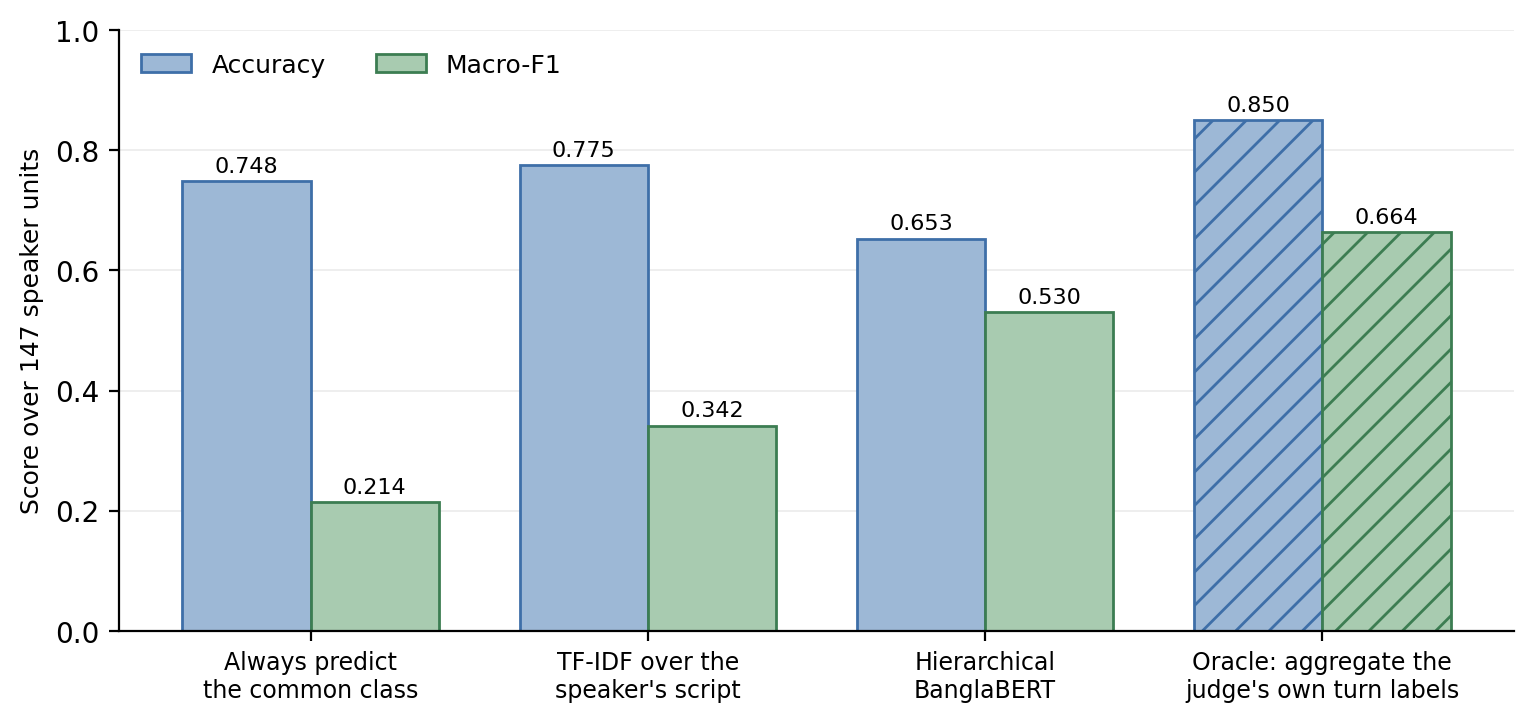
\includegraphics[width=0.92\textwidth]{figs/speaker_ladder.png}
\caption{Task B, the same four systems. Accuracy and macro-F1 move in opposite directions across
the ladder, which is why accuracy alone would rank the weakest system first. The hatched pair is
the oracle ceiling.}
\end{figure}

\vspace{2pt}
\textbf{The second route: aggregating Task A predictions.} A speaker verdict can also be reached
without a speaker model at all, by applying a fixed rule to the turn labels the Task A classifier
predicts. This is the route the shipped command-line scorer uses, and it is reported on the
30-unit held-out split so that it lines up with the Task A evaluation. Table~\ref{tab:aggrules} gives it. The
figures there look higher than Table~\ref{tab:taskb-systems} and are not comparable with it: 30 units against 147, a
single split against cross-validation, and a rule chosen on train+val rather than learned. It is
included because it is what the tool does, not as a rival measurement.

\begin{table}[htbp]\centering
\caption{Speaker-level results on the 30 valid test speaker units, by aggregation rule. The rule
was selected on the 117 train+val units, where \texttt{hard\_vote} won (exact accuracy 0.752), and
that rule is the one reported on test. \texttt{top\_k} transfers to a higher macro-F1, but quoting
it would be selection on the test set.}\label{tab:aggrules}
\begin{tabular}{|l|c|c|c|c|}
\hline
\thd{Aggregation rule} & \thd{Exact acc.} & \thd{Direction acc.} & \thd{Stance corr.} & \thd{Macro-F1} \\ \hline
\textbf{\texttt{hard\_vote}} (selected) & \textbf{0.867} & \textbf{0.867} & 0.451 & \textbf{0.567} \\ \hline
\texttt{top\_k}         & 0.800 & 0.800 & 0.628 & 0.667 \\ \hline
\texttt{word\_weighted} & 0.767 & 0.800 & 0.569 & 0.480 \\ \hline
\texttt{dur\_weighted}  & 0.767 & 0.800 & 0.567 & 0.480 \\ \hline
\texttt{unweighted}     & 0.633 & 0.667 & 0.691 & 0.447 \\ \hline
\end{tabular}
\end{table}

\begin{table}[htbp]\centering
\caption{Hierarchical speaker model (frozen turn encoder + attention pooling), out-of-fold over
\textbf{all 147 valid speaker units} under 5-fold \texttt{GroupKFold} grouped by episode. Because
every labelled speaker is used as test data exactly once, this is the speaker-level figure the
report quotes; the 30-unit held-out split in Table~\ref{tab:aggrules} is a sanity check, not a measurement.}
\begin{tabular}{|l|c|c|c|r|}
\hline
\thd{Class} & \thd{Precision} & \thd{Recall} & \thd{F1} & \thd{Units} \\ \hline
\texttt{negative} & 0.882 & 0.682 & 0.769 & 110 \\ \hline
\texttt{neutral}  & 0.519 & 0.778 & 0.622 & 18 \\ \hline
\texttt{positive} & 1.000 & 0.455 & 0.625 & 11 \\ \hline
\texttt{mixed}    & 0.067 & 0.250 & 0.105 & 8 \\ \hline
\multicolumn{5}{|l|}{\textbf{Overall: accuracy 0.653, macro-F1 0.530} (folds 0.500--0.828)} \\ \hline
\end{tabular}
\end{table}

\begin{figure}[htbp]\centering
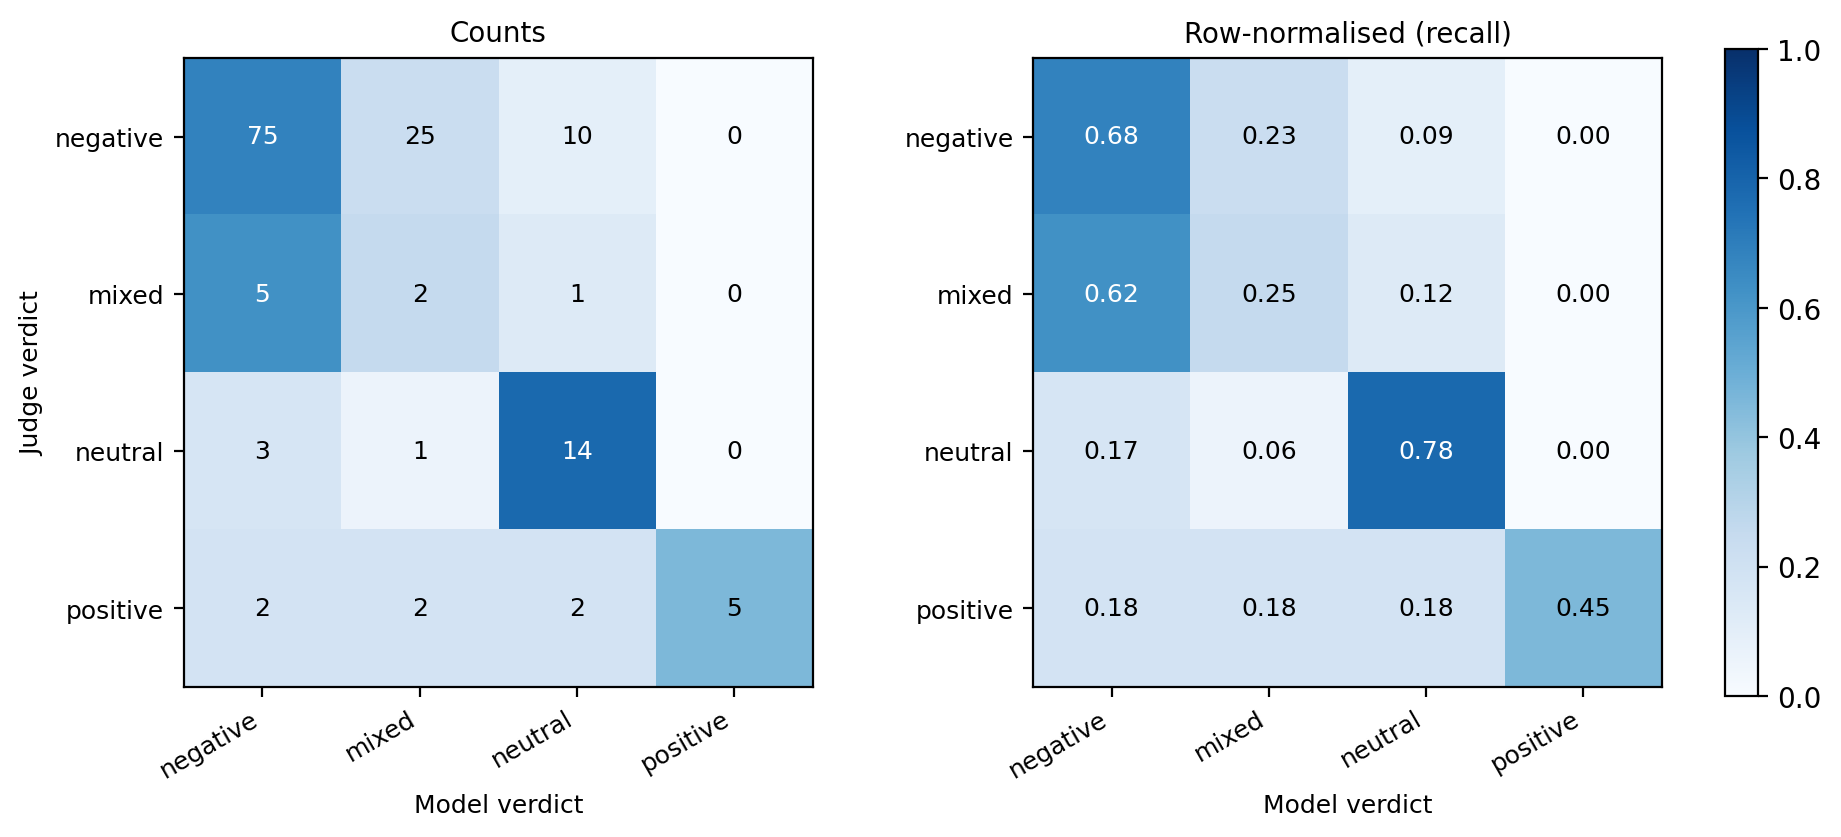
\includegraphics[width=0.96\textwidth]{figs/speaker_confusion.png}
\caption{Task B confusion matrix over the 147 out-of-fold speaker verdicts. The model never
labels a speaker \texttt{positive} unless it is right (precision 1.000), but it reaches only 45\%
of the positive speakers. The costly error is the opposite one: 25 genuinely negative speakers
are called \texttt{mixed}, which is the model hedging on a class it has only eight examples of.}
\end{figure}

\vspace{2pt}
\textbf{Where Task B fails.} Of 51 errors, exactly half (25) are \texttt{negative} speakers
called \texttt{mixed}. The \texttt{mixed} class is the problem: 8 training examples across the
whole corpus, an F1 of 0.105, and 30 predictions made where only 8 were warranted. It is
over-predicted because a speaker with any favourable turn at all looks mixed to the pooling
layer. The other direction is clean: no speaker is ever called \texttt{positive} wrongly, and
\texttt{neutral} recall is 0.778. Collapsing \texttt{mixed} into the polar classes would raise
the headline, so it is worth saying plainly that we did not do that. The class is small because
genuinely two-sided speakers are rare, not because the label is ill-defined, and Figure~\ref{fig:sample} shows
one being applied correctly.

\begin{table}[htbp]\centering
\caption{Task B accuracy and macro-F1 by slice. The model is weakest on the speakers who talk
most, which is the opposite of the Task A pattern and is consistent with the \texttt{mixed}
confusion above: the longer a speaker holds the floor, the more likely they say something
favourable somewhere, and the more likely the pooling layer hedges.}
\begin{tabular}{|l|r|c|c|}
\hline
\thd{Slice} & \thd{Units} & \thd{Accuracy} & \thd{Macro-F1} \\ \hline
\multicolumn{4}{|l|}{\textit{by inferred role}} \\ \hline
Host  & 45 & 0.689 & 0.463 \\ \hline
Guest & 101 & 0.644 & 0.381 \\ \hline
\multicolumn{4}{|l|}{\textit{by how much the speaker said}} \\ \hline
1--4 turns   & 28 & 0.643 & 0.531 \\ \hline
5--12 turns  & 74 & 0.662 & \textbf{0.607} \\ \hline
13+ turns    & 45 & 0.644 & 0.324 \\ \hline
\multicolumn{4}{|l|}{\textit{by transcript quality}} \\ \hline
\texttt{good} and \texttt{fair} & 144 & 0.660 & 0.542 \\ \hline
\texttt{poor}                   & 3 & 0.333 & 0.167 \\ \hline
\end{tabular}
\end{table}

\vspace{2pt}
\textbf{What the two tasks together say about the corpus.} Task A recovers turn sentiment at 0.670
macro-F1 against a 0.236 floor, so the turn labels are learnable. Task B recovers the speaker
verdict at 0.530 against a 0.214 floor, so the speaker labels are learnable too, and by a wider
relative margin, but it sits well under the 0.664 oracle. The distance between 0.530 and 0.664 is
what a better Task B model could still win by reading the turns more carefully; the distance
between 0.664 and 1.000 is what no turn-aggregation method can win at all, and is the part of the
speaker verdict that lives in the episode rather than in any single turn. Both figures are
agreement with the judge, not with human ground truth.

\vspace{2pt}
\textbf{Reproducing Task B.} \texttt{speaker\_level\_eval.py} recomputes every number in this
subsection, including the baselines, from the released out-of-fold predictions in about 15
seconds on CPU; \texttt{make\_speaker\_figs.py} redraws the two figures.

\textbf{The shipped scorer reproduces these numbers.} The command-line tool
\texttt{predict\_speakers.py} reads the rule, input mode and \texttt{max\_len} from
\texttt{metrics.json} so it cannot silently disagree with the notebook that trained the model.
Run end-to-end on CPU over the 324 held-out turns it recovers all 30 test speaker units and
reproduces the notebook's held-out figures exactly (exact accuracy 0.867 and stance
correlation 0.451 under the selected \texttt{hard\_vote} rule) in 47 seconds without a GPU.
All 324 turn-level predictions are identical to the ones the notebook wrote, which also shows
that the optional \texttt{csebuetnlp} normaliser is not load-bearing on this corpus: the CPU run
used the NFC fallback and still matched every label.

\emph{\small Briefly state what the baseline demonstrates about dataset usability. Avoid
over-interpreting performance.}

The baselines demonstrate that the corpus supports a valid supervised workflow at both levels. At
the turn level a standard Bangla encoder reaches macro-F1 0.670 against a 0.236 floor and a 0.529
non-neural reference, from 1{,}009 training turns under an episode-disjoint split, with
$\kappa=0.496$, which is moderate agreement with the judge on a three-class problem. At the speaker level,
aggregating those predictions reproduces the judge's verdict on 26 of 30 held-out speakers, and the
hierarchical model over all 147 units reaches 0.653 accuracy.

Four cautions belong with these numbers. First, \textbf{every score measures agreement with the LLM
judge, not with human ground truth}; macro-F1 0.670 means the student model reproduces the judge,
whose own accuracy is unmeasured. Second, \texttt{mixed} is not learnable at this scale: eight units
in the entire corpus give F1 0.105, and it should be treated as unsupported until the corpus grows.
Third, the speaker-level test split holds 30 units, so one unit moves macro-F1 by about 0.03 and the
gap between the selected and best-transferring aggregation rule is selection noise, not a finding.
Fourth, \textbf{the backbone ablation was not run}: BanglaBERT was adopted on published benchmark
evidence rather than compared on this corpus, and whether BanglishBERT handles the heavily
code-mixed financial vocabulary better remains an open question. The sweep is implemented in
Section 10 of the notebook behind a \texttt{RUN\_ABLATION} flag and costs about 25 GPU-minutes.

\section{Usage Notes and Reuse Potential}
%=======================================================================

\emph{\small Give practical instructions that help another student/researcher use the dataset
correctly.}

\begin{itemize}[leftmargin=1.4em,itemsep=3pt,topsep=2pt]
  \item \textbf{Loading.} Download the repository and read the JSONL files line by line
        (\texttt{json.loads} per line, UTF-8). For a model-ready corpus, use
        \texttt{turns\_\{train,val,test\}.jsonl} directly; no rebuild is needed. To re-derive
        from the fused bundles, run \texttt{build\_speaker\_corpus.py} ($\approx$20 s) then
        \texttt{make\_datasets.py} ($\approx$5 s).
  \item \textbf{Environment.} Python 3.10+, \texttt{torch} 2.12, \texttt{transformers},
        \texttt{scikit-learn}, \texttt{pandas}, \texttt{matplotlib}. Install the
        \texttt{csebuetnlp} normalizer, because BanglaBERT was pretrained on normalised text and the
        fallback to bare NFC costs measurable F1. On Windows, prefix commands with
        \texttt{python -X utf8} or the console encoder fails on Bangla.
  \item \textbf{Conventions.} \texttt{speaker\_id} is \textbf{episode-local}: \texttt{Speaker 0} in
        two episodes is not the same person. \texttt{asr\_confidence} is a mean log-probability, so
        it is negative and larger (closer to zero) is better. \texttt{stance\_score} runs from
        $-1$ (most negative) to $+1$ (most positive). Group on \texttt{global\_episode}, not on
        \texttt{roll} and not on \texttt{programme}.
  \item \textbf{Precautions.} Filter to \texttt{diarization\_trusted = true} for any claim about
        speaker attribution. Filter to \texttt{speaker\_level\_valid = true} for any speaker-level
        evaluation. Exclude \texttt{2107015::ep002} from programme-level claims (out of domain).
        Do not tune on the speaker-level validation split. It holds 23 units, and two of its
        four classes have only two members each, so use \texttt{GroupKFold} over all 147 valid
        units instead.
  \item \textbf{Reuse.} The retained audio supports acoustic and multimodal extensions (wav2vec2 /
        WavLM branches); the 52-target lexicon supports speaker $\times$ target aspect-based
        sentiment; the per-word ASR probabilities support ASR-robustness work on confusion
        networks; and the judged corpus supports LLM-judge calibration studies.
  \item \textbf{Inappropriate uses.} Do not present model output as the identified opinion of a
        named individual, because speaker IDs are clustering predictions, not identities. Do not quote
        the macro-F1 figures as human-validated accuracy. Do not use this corpus to make trading or
        policy decisions without the human-verification step in Section 12.
\end{itemize}

%=======================================================================
\section{Limitations and Known Biases}
%=======================================================================

\emph{\small Recommended: up to about 200 words. Discuss limitations of the dataset itself: sample
size, coverage, imbalance, acquisition constraints, label uncertainty, measurement error,
missingness, bias, or restricted generalizability. Do not hide limitations.}

\textbf{No human labels exist.} All supervision comes from a single LLM judging pass, so
\texttt{pass\_agreement} is 1.0 by construction and no self-consistency or inter-annotator figure
can be quoted. The judge and any model trained on it share a blind spot: if the judge over-reads
negativity in garbled text, the student learns to do the same, and no evaluation against judge
labels will reveal it.

\textbf{Three core quality metrics are unmeasured.} Word error rate, diarization error rate and
annotation $\kappa$ are all recorded as \texttt{SKIPPED} for want of gold references. The
literature places the comfortable ceiling for sentiment on ASR output near 12\% WER; this ASR is
visibly worse, with invented words, dropped inflections and wrong numbers.

\textbf{Scale and coverage.} One hundred and forty-seven valid speaker units and 1{,}630
supervised turns remain small for a four-class speaker task; one unlucky episode still moves a
held-out score by about three points, so grouped cross-validation and seed averaging are required
before quoting a figure as final. \texttt{positive} and \texttt{mixed} number only 11 and 8
speaker units in the entire corpus. A majority of episodes carry placeholder or empty programme
titles, which prevents the stricter programme-level split. Two episodes contain out-of-domain
material and are excluded by labelling rather than deletion. The corpus is negative-dominant
(53\%), partly because the period genuinely was, with a banking crisis, an energy shock and
sustained inflation, and partly through selection; these explanations are separable only by
the human-verification sample.

\textbf{Two build-1 limitations have been removed} and are recorded here for transparency rather
than deleted: roll \texttt{2107009}'s fallback diarization (five episodes, 60--70\% of words
unattributed) has been replaced by \texttt{pyannote}, and the speaker-level validation split that
previously held six units across two classes now holds 23 across four.

%=======================================================================
\section{Ethics, Privacy and Responsible Data Use}
%=======================================================================

\emph{\small Complete the applicable items. If human participants or personal data are involved,
state consent/approval/anonymization details. If data come from social media/web platforms,
address terms of service and redistribution. If none apply, state that explicitly.}

\begin{longtable}{|L{4.4cm}|L{11.0cm}|}
\hline
\thd{Human participants / consent} & Not applicable. No human participants were recruited and no
experiment was conducted. All speakers are public figures appearing voluntarily on broadcast
television in a professional capacity. No ethics-board approval was sought or required for
analysis of publicly broadcast material. \\ \hline
\thd{Privacy / de-identification} & Speakers are released only as episode-local cluster indices
(\texttt{Speaker 0}, \texttt{Speaker 1}, \dots) and are not linked to names. No personal
identifiers, contact details or non-public information are stored. Speaker identity is a model
prediction, not an assertion about a real person, and downstream users are instructed not to
present it as one. \\ \hline
\thd{Web / social-media data} & Not applicable in the social-media sense; the material is
television broadcast audio obtained from public platform postings. Episodes were downloaded from publicly posted broadcast uploads with a standard command-line downloader and converted to 16\,kHz mono WAV locally. \textbf{Compliance with each platform's terms of service has not been formally verified}, which is precisely why the audio is not redistributed and every \texttt{license\_attestation} field still reads \texttt{UNVERIFIED}. \\ \hline
\thd{Copyright / third-party data} & Source audio is third-party copyrighted broadcast content.
\textbf{The audio is not redistributed.} The release contains derived artefacts (transcripts,
timings, speaker segments and annotations) together with the episode registry (titles,
channels, durations, SHA-256) so that a user can obtain the source independently.
The derived annotations are released under CC BY 4.0; each episode's originating channel (RTV Business, ATN Bangla, and 11 episodes whose channel is recorded as \texttt{unknown}) is attributed in \texttt{registry.csv}. The \texttt{license\_attestation} field in every registry row currently reads
\texttt{UNVERIFIED} and must be completed before public release. \\ \hline
\thd{AI-generated / synthetic content} & \textbf{Disclosed.} No synthetic data were generated, but
\textbf{all sentiment labels are AI-generated}: 100\% of the 1{,}811 turn labels and all 150
speaker verdicts were produced by Claude Opus 5 under a human-authored rubric, in a single
pass. Human effort went into curation rather than labelling, covering rubric design,
diarization repair, unit screening, out-of-domain exclusion and the discarding of stale blocks,
all itemised with counts in Section~5.5. \textbf{No human annotator re-labelled individual turns}, and the
annotation drafts in the roll folders still record \texttt{human\_verified: false} for all 5{,}395
prepared utterances. Transcripts are machine-generated by Whisper-medium and speaker
segments by \texttt{pyannote}. Every score in this report is agreement with an AI judge, not with
human truth. \\ \hline
\end{longtable}
% This longtable has no caption, so it must not consume a table number.
\addtocounter{table}{-1}

%=======================================================================
\section{Data and Code Availability}
%=======================================================================

\begin{longtable}{|L{4.6cm}|L{10.8cm}|}
\hline
\thd{Item} & \thd{Details} \\ \hline
\endfirsthead
\hline \thd{Item} & \thd{Details} \\ \hline \endhead
\thd{Repository name}                   & GitHub: {\scriptsize\texttt{mayer-doa-coder/bangla-financial-talkshow-sentiment}}; Zenodo is the intended archival host once a DOI is minted \\ \hline
\thd{Dataset DOI / persistent identifier} & Not yet minted \\ \hline
\thd{Direct dataset URL}                & {\scriptsize\url{https://github.com/mayer-doa-coder/bangla-financial-talkshow-sentiment}} \\ \hline
\thd{Access instructions}               & Restricted to the course instructor at submission; intended to become public. Derived annotations and transcripts are released; source broadcast audio is not redistributed and is obtainable from the channel references in \texttt{registry.csv}. \\ \hline
\thd{Dataset license}                   & CC BY 4.0 for the derived annotations, transcripts and timings \emph{only}. Source broadcast audio is third-party copyrighted and is not covered by this licence and not redistributed (Section 13). \\ \hline
\thd{Code / notebook URL}               & Same repository, under \texttt{speaker\_sentiment/}. Contains \texttt{build\_speaker\_corpus.py}, \texttt{llm\_judge.py}, \texttt{make\_datasets.py}, \texttt{predict\_speakers.py}, \texttt{tfidf\_baseline.py} and \texttt{Speaker\_Sentiment\_BanglaBERT.ipynb}. \\ \hline
\thd{Code version / commit / release}   & v1.0, build 2 (45-episode corpus); the archive is not under version control, so the release is identified by the dataset version \\ \hline
\thd{README \& environment}             & \texttt{speaker\_sentiment/README.md} (pipeline, caveats, exact run sequence); \texttt{speaker\_sentiment/requirements.txt}; \texttt{torch} 2.12, \texttt{transformers}, \texttt{scikit-learn}, \texttt{pandas}, \texttt{matplotlib} \\ \hline
\end{longtable}
% This longtable has no caption, so it must not consume a table number.
\addtocounter{table}{-1}

%=======================================================================
\section{Student Contributions (CRediT-style)}
%=======================================================================

\emph{\small Report contributions transparently. Each student should have a clear role. Typical
roles include conceptualization, methodology, data curation, investigation, software, validation,
formal analysis, visualization, writing, and project administration.}

\vspace{2pt}
Two figures are reported per student because they answer different questions. \textbf{Data share}
is measured, not negotiated: it is the mean of each student's share of episodes, speaker turns and
transcribed words in the released corpus, computed directly from \texttt{turns.jsonl} and
\texttt{speakers.jsonl}, and it is reproducible from the files in the archive. It is uneven because
episode availability was uneven, and some programmes published far more usable broadcasts
than others. \textbf{Overall share} is the team's agreed division of the whole workload, which includes
the pipeline engineering, annotation-draft preparation, diarization repair, modelling, analysis
and report writing that the data share cannot see. Students with smaller collections carried
correspondingly more of that shared work, which is why the overall column is close to even; the
role column below records which parts each student took. The evidence column is the
machine-verifiable part of the claim.

\begingroup\footnotesize
\begin{longtable}{|L{1.3cm}|L{2.9cm}|L{1.0cm}|L{1.0cm}|L{4.1cm}|L{3.3cm}|}
\hline
\thd{Roll} & \thd{Student} & \thd{Data share (\%)} & \thd{Over-all (\%)} & \thd{CRediT roles and what they covered} & \thd{Evidence / files owned} \\ \hline
\endfirsthead
\hline \thd{Roll} & \thd{Student} & \thd{Data share (\%)} & \thd{Over-all (\%)} & \thd{CRediT roles and what they covered} & \thd{Evidence / files owned} \\ \hline \endhead
2107001 & Nafiz Ahmed & 9.4 & 16.0 &
\emph{Data curation; methodology; validation; investigation; writing (review and editing).}
Collection and pipeline run for roll 2107001; audio hygiene and the 16\,kHz mono preprocessing
tier; weak-supervision and GER trial branches; co-author of the six genre-specific rubric rules
and reviewer of the rubric's borderline cases &
\texttt{2107001/results/}: 4 episodes, 2.7\,h, 239 turns, 20{,}670 words, 12 judged units, 184
turn labels; the only bundle carrying a complete \texttt{processed/}, \texttt{weak/} and
\texttt{ger/} tier (37 files, 714\,MB) \\ \hline
2107004 & Tawhidul Hasan & 21.7 & 17.0 &
\emph{Software; data curation; conceptualization; project administration; writing (review
and editing).} Collection and pipeline run for roll 2107004; the corpus-build, judge-merge and
split scripts; cross-roll consolidation of six differing folder layouts into one schema &
\texttt{2107004/results/}: 10 episodes, 5.6\,h, 570 turns, 42{,}622 words, 29 judged units, 425
turn labels; \texttt{CONSOLIDATION.md},\newline \texttt{aggregated/}\newline\texttt{STATUS.md}, 10 annotation drafts,
\texttt{weak\_labels/} (84 files) \\ \hline
2107006 & Sarwad Hasan Siddiqui & 30.1 & 17.5 &
\emph{Conceptualization; methodology; formal analysis; writing (original draft); project
administration; data curation.} Largest collection share; annotation rubric and the
out-of-domain exclusion criteria; report preparation; corresponding student &
\texttt{2107006/results/}: 14 episodes, 9.4\,h, 625 turns, 73{,}091 words, 60 judged units, 459
turn labels; 8 \texttt{aggregated/} quality-gate files (143 files, 828\,MB) \\ \hline
2107009 & Saif Ahmed Shejan & 9.8 & 16.0 &
\emph{Validation; data curation; investigation; writing (review and editing).} Collection and
pipeline run for roll 2107009; the diarization quality audit that identified build~1's worst
defect and the \texttt{pyannote} re-run that repaired it, turning 263 unusable fragments on
\texttt{ep001} into 47 real speaker turns &
\texttt{2107009/results/}: 5 episodes, 2.8\,h, 190 turns, 22{,}498 words, 15 judged units, 151
turn labels; 15 diarization artefacts over 5 episodes (three passes per episode) \\ \hline
2107010 & Maruf Shafiq & 10.0 & 16.0 &
\emph{Visualization; formal analysis; data curation; writing (original draft) (results);
investigation.} Collection and pipeline run for roll 2107010; the confusion matrix, per-class
and role/transcript-quality breakdowns; the qualitative error analysis behind Section~11 &
\texttt{2107010/Results/}: 4 episodes, 2.7\,h, 289 turns, 20{,}131 words, 11 judged units, 205
turn labels; 18 diarization artefacts over 4 episodes; \texttt{annotated/},
\texttt{weak\_labels/} \\ \hline
2107015 & Dewan Salman Rahman Zisan & 19.0 & 17.5 &
\emph{Software; formal analysis; visualization; data curation; writing (review and editing).}
Collection and pipeline run for roll 2107015; BanglaBERT fine-tuning, the aggregation-rule study
and the hierarchical speaker model; the corpus diversity audit &
\texttt{2107015/results/}: 8 episodes, 5.3\,h, 501 turns, 40{,}264 words, 23 judged units, 387
turn labels; \texttt{models/}, \texttt{artifacts/}, \texttt{reports/}\newline\texttt{diversity\_audit.md} and 5
report figures \\ \hline
\end{longtable}
% This longtable has no caption, so it must not consume a table number.
\addtocounter{table}{-1}

%=======================================================================
\section{Acknowledgements, Funding and Competing Interests}
%=======================================================================

\subsection{Acknowledgements / Funding}

{\sloppy We acknowledge the course instructors of CSE 4112 for guidance, and the authors of
\texttt{csebuetnlp/\allowbreak banglabert}, \texttt{pyannote.\allowbreak audio} and the BengaliAI
Whisper-medium ASR model, whose openly released models made this pipeline possible.\par}
This work received no external funding.

\subsection{Declaration of Competing Interests}

The authors declare no competing interests relevant to this dataset report.

%=======================================================================
\section{References}
%=======================================================================

\emph{\small Use numbered references in order of citation. Include sources for the problem domain,
data-collection/measurement method, data source(s), instruments/software, related datasets, and
any ML baseline methods that are actually used. A concise list (typically $\le$20 references) is
sufficient for a data-focused report.}

\begin{thebibliography}{99}\setstretch{1.0}\small

\bibitem{banglabert} A. Bhattacharjee, T. Hasan, W.~U. Ahmad, K.~S. Mubasshir, M.~S. Islam,
A. Iqbal, M.~S. Rahman, and R. Shahriyar, ``BanglaBERT: Language model pretraining and benchmarks
for low-resource language understanding evaluation in Bangla,'' in \emph{Findings of NAACL 2022},
2022. arXiv:2101.00204.

\bibitem{blp2023} Organizers and participants, ``BLP-2023 Task 2: Sentiment analysis of Bangla
social media posts,'' in \emph{Proc.\ 1st Workshop on Bangla Language Processing}, 2023.

\bibitem{banabsa} M.~M. Rahman and E. Kabir, ``BAN-ABSA: An aspect-based sentiment analysis
dataset for Bengali and its baseline evaluation,'' in \emph{Proc.\ Int.\ Joint Conf.\ on Advances
in Computational Intelligence}, Springer, 2021.

\bibitem{babsa} Authors, ``BABSA: A large-scale Bangla aspect-based sentiment analysis dataset,''
\emph{Data in Brief}, 2026.

\bibitem{erc} S. Poria, D. Hazarika, N. Majumder, G. Naik, E. Cambria, and R. Mihalcea,
``MELD: A multimodal multi-party dataset for emotion recognition in conversations,'' in
\emph{Proc.\ ACL}, 2019.

\bibitem{earnings} Authors, ``Advanced deep learning techniques for analyzing earnings call
transcripts,'' arXiv:2503.01886, 2025.

\bibitem{pyannote} H. Bredin \emph{et al.}, ``pyannote.audio: Neural building blocks for speaker
diarization,'' in \emph{Proc.\ ICASSP}, 2020. Model:
\texttt{pyannote/speaker-diarization-community-1}.

\bibitem{whisper} A. Radford, J.~W. Kim, T. Xu, G. Brockman, C. McLeavey, and I. Sutskever,
``Robust speech recognition via large-scale weak supervision,'' in \emph{Proc.\ ICML}, 2023.
Fine-tuned checkpoint: \texttt{bengaliAI/tugstugi\_bengaliai-asr\_whisper-medium}.

\bibitem{hierarch} J. Li, D. Ji, F. Li, M. Zhang, and Y. Liu, ``HiTrans: A transformer-based
context- and speaker-sensitive model for emotion detection in conversations,'' in
\emph{Proc.\ COLING}, 2020. arXiv:2012.14781.

\bibitem{llmjudge} Z. Tan \emph{et al.}, ``Large language models for data annotation and
synthesis: A survey,'' arXiv:2402.13446, 2024.

\bibitem{asrglue} L. Feng \emph{et al.}, ``ASR-GLUE: A new multi-task benchmark for ASR-robust
natural language understanding,'' arXiv:2108.13048, 2021.

\bibitem{wersent} Authors, ``Speech emotion recognition with ASR transcripts: A comprehensive
study on word error rate and fusion techniques,'' arXiv:2406.08353, 2024.

\bibitem{thisdataset} N. Ahmed, T. Hasan, S.~H. Siddiqui, S.~A. Shejan, M. Shafiq, and
D.~S.~R. Zisan, ``A speaker-attributed sentiment dataset for Bangla financial television talk
shows,'' v1.0, Department of CSE, Khulna University of Engineering \& Technology, 2026.
GitHub: mayer-doa-coder/bangla-financial-talkshow-sentiment. DOI not yet minted.

\end{thebibliography}

%=======================================================================
%  APPENDICES
%=======================================================================
\clearpage

\section*{\sffamily Appendix A. Complete Data Dictionary (if needed)}

\emph{\small Place the full variable/field dictionary here if Section 7.2 would otherwise become
too long.}

\textbf{A.1 \texttt{turns.jsonl}: 2{,}414 rows, 19 fields}

\begin{longtable}{|L{3.4cm}|L{2.0cm}|L{9.6cm}|}
\hline
\thd{Field} & \thd{Type} & \thd{Definition} \\ \hline
\endfirsthead
\hline \thd{Field} & \thd{Type} & \thd{Definition} \\ \hline \endhead
\texttt{turn\_id}               & string  & \texttt{roll::episode::turnNNNN}, globally unique \\ \hline
\texttt{roll}                   & string  & Collecting student's roll number \\ \hline
\texttt{episode}                & string  & Episode identifier local to the roll (\texttt{epNNN}) \\ \hline
\texttt{global\_episode}        & string  & \texttt{roll::episode}; \textbf{the grouping key for all splits} \\ \hline
\texttt{turn\_index}            & integer & Ordinal position of the turn within the episode \\ \hline
\texttt{speaker\_id}            & integer & Diarization cluster index, episode-local; $-1$ = unassigned \\ \hline
\texttt{start\_sec}, \texttt{end\_sec}, \texttt{dur\_sec} & float & Turn boundaries and duration, seconds \\ \hline
\texttt{text}                   & string  & Normalised Bangla transcript \\ \hline
\texttt{text\_raw}              & string  & Transcript before normalisation \\ \hline
\texttt{n\_words}               & integer & Whitespace word count \\ \hline
\texttt{n\_windows}             & integer & Number of ASR decode windows merged into this turn \\ \hline
\texttt{asr\_confidence}        & float   & Mean log-probability over the turn's words ($\le 0$) \\ \hline
\texttt{diarization\_provider}  & string  & \texttt{pyannote} or \texttt{fallback} \\ \hline
\texttt{diarization\_trusted}   & boolean & True for all 45 episodes in this build \\ \hline
\texttt{flag\_repetition\_loop} & boolean & ASR degenerate-repetition failure detected \\ \hline
\texttt{flag\_too\_short}       & boolean & Turn below the minimum usable length \\ \hline
\texttt{role}                   & string  & \texttt{host} / \texttt{guest} / \texttt{minor} / \texttt{unassigned} \\ \hline
\end{longtable}
% This longtable has no caption, so it must not consume a table number.
\addtocounter{table}{-1}

\textbf{A.2 \texttt{speakers.jsonl}: 212 rows.} Adds \texttt{speaker\_key}, \texttt{programme},
\texttt{n\_turns}, \texttt{n\_usable\_turns}, \texttt{n\_words}, \texttt{n\_clean\_words},
\texttt{dur\_sec}, \texttt{mean\_words\_per\_turn}, \texttt{n\_loop\_turns},
\texttt{mean\_asr\_confidence}, \texttt{script} (concatenated turns), \texttt{turn\_ids} and
\texttt{judgeable}.

\textbf{A.3 \texttt{judgements.jsonl}: 150 rows.} \texttt{pass\_id}, \texttt{judge\_model},
\texttt{speaker\_label}, \texttt{stance\_score}, \texttt{speaker\_confidence},
\texttt{speaker\_summary}, \texttt{speaker\_rationale}, \texttt{dominant\_topics},
\texttt{transcript\_quality}, \texttt{n\_turns\_sent}, \texttt{n\_turns\_returned},
\texttt{turn\_labels} (list of \{\texttt{turn\_id}, \texttt{label}, \texttt{confidence},
\texttt{evidence}\}) and \texttt{usage}.

\textbf{A.4 \texttt{speakers\_labelled.jsonl}: 150 rows.} Adds \texttt{speaker\_level\_valid},
per-class counts, \texttt{net\_polarity}, \texttt{net\_polarity\_word\_weighted}, the five
aggregation outputs (\texttt{agg\_majority\_vote}, \texttt{agg\_net\_polarity},
\texttt{agg\_word\_weighted}, \texttt{agg\_conf\_weighted}, \texttt{agg\_word\_conf\_weighted})
and \texttt{split}.

\textbf{A.5 \texttt{turns\_\{train,val,test\}.jsonl}: 1{,}009 / 297 / 324 rows.} Turn fields plus
\texttt{speaker\_key}, \texttt{label}, \texttt{judge\_confidence}, \texttt{evidence},
\texttt{n\_passes}, \texttt{pass\_agreement}, \texttt{weight} and \texttt{split}.

\textbf{A.6 \texttt{registry.csv}: 32 rows.} \texttt{episode\_id}, \texttt{channel},
\texttt{duration\_sec}, \texttt{programme}, \texttt{has\_remote\_guest},
\texttt{covers\_market\_news}, \texttt{local\_path}, \texttt{sha256},
\texttt{license\_attestation}, \texttt{sample\_rate}, \texttt{channels}, \texttt{codec},
\texttt{bit\_rate\_kbps}, \texttt{file\_size\_bytes}, \texttt{duration\_flag},
\texttt{rejection\_reason}, \texttt{sha256\_verified}, \texttt{notes}.

\vspace{8pt}
\section*{\sffamily Appendix B. Optional Supporting Material}

\begin{itemize}[leftmargin=1.4em,itemsep=2pt,topsep=2pt]
  \item Representative raw samples: an excerpt of a fused episode JSON showing word-level timings,
        probabilities and speaker assignment, alongside the reconstructed turn.
  \item Screenshots of the retrieval demonstration application (\texttt{demo/app.py}), which
        indexes every roll bundle and exposes speaker-filtered exact, fuzzy, semantic and hybrid
        search over the corpus with playable audio excerpts.
  \item Labelling guideline: the full judge rubric with worked annotation examples for each of the
        six genre-specific rules.
  \item Additional validation tables: the aggregation-rule agreement study (five rules, bottom-up
        vs.\ top-down), the subword length distribution used to choose \texttt{max\_len}, and the
        per-episode diarization-provider breakdown.
  \item Environment specification and reproducibility notes: model revision hashes, seeds
        (pipeline 17, modelling 7), and measured CPU/GPU timings.
  \item The financial-target taxonomy (52 canonical targets with stems and orientation) and the
        103-entry polarity-cue lexicon.
\end{itemize}

\vspace{4pt}
{\small\emph{Template basis: Data in Brief data-article structure; Scientific Data Data Descriptor
structure; MDPI Data Data Descriptor structure; plus CSE 4112-specific ML workflow and
leakage-control requirements.}}

\vspace{8pt}
\section*{\sffamily Appendix C. Dataset Release and FAIR-Readiness Checklist}

\begingroup\footnotesize
\begin{longtable}{|L{2.9cm}|L{6.4cm}|L{2.3cm}|L{3.4cm}|}
\hline
\thd{Checklist item} & \thd{Criterion} & \thd{Yes/No} & \thd{Evidence / note} \\ \hline
\endfirsthead
\hline \thd{Checklist item} & \thd{Criterion} & \thd{Yes/No} & \thd{Evidence / note} \\ \hline \endhead
\thd{Findable}       & Repository and persistent identifier/URL are provided; file/folder names are meaningful; metadata are searchable. & $\boxtimes$~Yes~/~$\square$~No & GitHub: \texttt{mayer-}\newline\texttt{doa-coder/}\newline\texttt{bangla-financial-}\newline\texttt{talkshow-}\newline\texttt{sentiment}\newline{}DOI at archival release. \\ \hline
\thd{Accessible}     & Access instructions work; restrictions are justified; files can be downloaded by the intended user. & $\boxtimes$~Yes~/~$\square$~No & Audio not redistributed; \texttt{registry.csv} enables independent retrieval \\ \hline
\thd{Interoperable}  & Common/open formats and standard units/labels are used where possible; schemas/codings are documented. & $\boxtimes$~Yes~/~$\square$~No & JSON / JSONL / CSV / WAV / RTTM; fused schema 2.0; Appendix A \\ \hline
\thd{Reusable}       & License is explicit; README, data dictionary, provenance, limitations and citation information are provided. & $\boxtimes$~Yes~/~$\square$~No & CC BY 4.0 (derived annotations); README, Appendix A, Sections 9 and 12 present \\ \hline
\thd{Raw + processed separation} & Original observations are preserved separately from cleaned/derived data. & $\boxtimes$~Yes~/~$\square$~No & Raw audio kept unmodified locally and excluded from the repository (Section 13); derived artefacts under \texttt{results/} \\ \hline
\thd{Versioning}     & Dataset version/date and change history are recorded. & $\boxtimes$~Yes~/~$\square$~No & v1.0, 15 September 2026; build 1 $\rightarrow$ build 2 changes recorded in Section 4 \\ \hline
\thd{Integrity}      & Duplicate/corruption/schema checks are complete; checksums are included where useful. & $\boxtimes$~Yes~/~$\square$~No & SHA-256 in \texttt{registry.csv} and \texttt{run\_manifest.json}; transcript-hash dedup \\ \hline
\thd{Leakage safety} & Related samples/subjects/augmentations do not cross ML data partitions. & $\boxtimes$~Yes~/~$\square$~No & Episode-disjoint split asserted in code; \textbf{programme-level overlap remains} (Section 12) \\ \hline
\thd{Reproducible processing} & Code/notebook can reproduce processed data and baseline pipeline from the released inputs. & $\boxtimes$~Yes~/~$\square$~No & \texttt{build\_speaker\_corpus.py} + \texttt{make\_datasets.py} + notebook; seeds 17 / 7 \\ \hline
\thd{Ethics/privacy} & Consent/approval/licensing/anonymization requirements are satisfied. & $\square$~Yes~/~$\boxtimes$~No & Episode-local speaker indices only, but \texttt{license\_attestation} is still \texttt{UNVERIFIED} for all 56 rows \\ \hline
\thd{Documentation}  & README explains files, variables, setup and reuse; captions/tables match the repository contents. & $\boxtimes$~Yes~/~$\square$~No & \texttt{speaker\_sentiment/}\newline\texttt{README.md} \\ \hline
\thd{Team accountability} & All six students' contributions are recorded. & $\boxtimes$~Yes~/~$\square$~No & Section 15 \\ \hline
\end{longtable}
% This longtable has no caption, so it must not consume a table number.
\addtocounter{table}{-1}
\endgroup

\end{document}
